\chapter{Introdução}
\label{cap:introducao}

Atualmente, as crianças e jovens brasileiros possuem cada vez mais acesso e contato
com tecnologias digitais. Cerca de 75\% dos jovens entre 10 e 18 anos afirmam navegar na internet, e 38,3\% afirmam que a utilizam para estudos e realização de tarefas escolares \cite{escola_futuro:2012}. Além disso, de acordo com o New Horizon Report \cite{horizon:2012}, mundialmente, as instituições de ensino aumentam cada vez mais a disponibilidade e a qualidade de acesso à internet dentro de suas dependências.

Os estudantes também trazem cada vez mais seus próprios dispositivos para as salas de aula, em um movimento conhecido como \emph{Bring Your Own Device} (BYOD), como \emph{notebooks}, \emph{tablets} e \emph{smartphones}, dispositivos estes que também são utilizados para seus estudos fora de sala de aula. Esses dispositivos poderiam enriquecer o aprendizado independente de lugar e momento, não restringindo a somente as salas de aula \cite{horizon_k12:2014}. 

%A presença massiva de tecnologia na vida de alunos e professores propícia a utilização de sistemas computacionais educacionais independente do mesmo estar dentro ou fora de sala de aula.


Além da presença de tecnologia em sala de aula ocorrer naturalmente por parte dos alunos como visto anteriormente, existem ações públicas em diversos países que visam à inclusão de tecnologia tanto para alunos quanto para professores. O governo brasileiro, por exemplo, por meio do programa ProInfo fomenta o uso de tecnologia da informação e comunicação (TIC) na rede pública de ensino \cite{proinfo}. Essa presença de infraestrutura favorece cada vez mais a utilização de sistemas computacionais para a educação.

Os sistemas para educação vem evoluindo juntamente com a computação, e tem como objetivo atuar como meio ou ferramenta a contribuir com objetivos pedagógicos \cite{tchounikine11}. Atualmente a utilização de sistemas computacionais podem ocorrer em todos os aspectos do ambiente educacional servindo assim vários propósitos e objetivos. Alguns propósitos utilizados atualmente incluem servir realmente como um meio de instrução, onde o aprendizado acontece completamente por meio de computadores \cite{mlearning09}, ou ainda no uso da gestão da educação, propiciando novos recursos para que professores e demais envolvidos no processo possuam dados e ferramentas para acompanhamento do progresso dos alunos \cite{flescher02} ou ainda com o enriquecimento da experiência de aprendizagem por meio de recursos computacionais \cite{cotton91}. A computação em sala de aula está abrindo novas possibilidades de utilização de metodologias pedagógicas que sem tecnologia eram impraticáveis ou inviáveis. Um exemplo de metodologia potencializada pela tecnologia é a Sala de Aula Invertida. 

A Sala de Aula Invertida é uma metodologia onde lições teóricas são realizadas online por meio da internet e o tempo em sala de aula é utilizado para tirar dúvidas e para aplicação destas teorias em trabalhos práticos que podem envolver o trabalho conjunto entre os alunos \cite{staker_classifying_2012}. A utilização de metodologias inovadoras em conjunto com atividades que envolvem dois ou mais alunos colaborando por um objetivo em comum aumentam e muito sua motivação.

A motivação é um dos aspectos educacionais bastante pesquisados atualmente principalmente pelos benefícios ao processo. Estudos apontam que quando os alunos participam ativamente do processo, esta atividade acaba por aumentar o aprendizado e persistência do mesmo, aumentam as notas ou ainda torna-os mais participativos \cite{felder1992quick}. Assim, torna-se relevante a pesquisa de sistemas computacionais que poderiam ser utilizados na educação para aproveitar o ambiente que já conta com dispositivos conectados à internet dos próprios alunos ou fornecidos pelas escolas, porém sua utilização poderia ser diferente da realizada atualmente. Atualmente, muitos sistemas educacionais são utilizados somente como meio de transferência de materiais de aula e tem funcionalidades relacionadas a colaboração sub-utilizadas \cite{fulano}.

Neste contexto, foram elaboradas as seguintes perguntas de pesquisa para este trabalho:

\textbf{Pergunta 1:} quais seriam as funcionalidades interessantes a um possível sistema colaborativo a ser utilizado durante e após a aula?

\textbf{Pergunta 2:} considerando estes requisitos e considerando que o sistema possa ser utilizado em várias plataformas e dispositivos, quais as tecnologias poderiam ser utilizadas em seu desenvolvimento?

Como hipótese inicial a Pergunta de Pesquisa 1 temos o seguinte conjunto de funcionalidades:

\textbf{Funcionalidade 1:} permitir ao aluno visualizar conteúdo (apresentações, textos, vídeos, etc) disponibilizado pelo professor, tanto durante a aula quanto depois dela;

\textbf{Funcionalidade 2:} possibilitar ao aluno informar anonimamente o professor, durante a aula, o quanto está compreendendo o assunto;

\textbf{Funcionalidade 3:} possibilitar que o professor receba o retorno dado pelo aluno na funcionalidade anterior em tempo real, enquanto está dando aula, sobre o quanto os alunos julgam estar entendendo o conteúdo. Permitir também que o professor visualize o histórico destes retornos;

\textbf{Funcionalidade 4:} permitir que o aluno faça anotações no computador ou em dispositivos móveis diretamente sobre o material de aula que o professor disponibilizou;

\textbf{Funcionalidade 5:} permitir ao aluno compartilhar estas anotações (descritas na funcionalidade anterior) e dúvidas, respostas ou comentários com os demais alunos, durante a aula e depois dela;

A validação dessa hipótese será realizada através de uma pesquisa com alunos e professores do ensino médio e superior, onde cada um destes grupo de usuários respondeu sobre a relevância destas funcionalidades a um futuro sistema a ser desenvolvido, a metodologia dessa pesquisa foi descrita na Seção \ref{sec:metodologia_professores}. Outra análise também avaliou as funcionalidades presentes em sistemas educacionais comerciais e descritas em artigos científicos, estas funcionalidades foram levantadas e analisadas através da revisão da literatura descrita no Capítulo \ref{chap:revisao}. O sistema desenvolvido contendo estas funcionalidades também foi utilizado em um experimento para conhecer a relevância como um todo no processo de ensino e aprendizagem. O experimento foi realizado conforme descrito na Seção \ref{sec:metodologia_experimento} e seus resultados compõe o Capítulo \ref{cap:resultados}.

Já as hipóteses iniciais para a segunda pergunta de pesquisa que envolve a definição das tecnologias mais adequadas para o desenvolvimento incluem dois grupos de tecnologias: uma onde a interface com o usuário utilizaria Java Applet e outra onde seria utilizado HTML5, JavaScript e CSS3. A validação de cada hipótese será realizada através de um experimento realizado no LInE, onde foi possível coletar indícios de facilidade de execução pelo usuário final em cada uma delas. Será utilizado também relatos e estudos de casos disponibilizados publicamente. A metodologia do experimento realizado no LInE é descrito na Seção \ref{sec:metodologia_line} já seus resultados são descritos na Seção \ref{sec:tecnologias_frontend}.

Assim, o objetivo geral deste trabalho é definir um conjunto de funcionalidades para um sistema a ser utilizado durante a aula e após a mesma e quais as tecnologias mais adequadas para seu desenvolvimento. Como objetivos secundários será avaliado a utilização deste sistema e também sua usabilidade, além da opinião dos alunos na utilização da metodologia da Sala de Aula Invertida para um curso de programação. A seguir é apresentado como este trabalho está organizado.

\section{Organização do documento}

Neste Capítulo introduzimos sobre o escopo ao qual este trabalho está relacionado e definimos as perguntas de pesquisa e o objetivo do trabalho. No Capítulo \ref{cap:fundamentacao} é apresentado os conceitos envolvidos no trabalho através da Fundamentação Teórica. Já o Capítulo \ref{cap:metodologia} apresenta a metodologia aplicada no trabalho e em cada experimento realizado. 

No Capítulo \ref{chap:revisao} é realizada a revisão da literatura para conhecer outros sistemas comerciais e acadêmicos que podem ser utilizados para a educação. No Capítulo \ref{cap:mindboard} é descrito como foi desenvolvido o sistema Mindboard, quais tecnologias foram utilizadas e todas as demais decisões técnicas. Neste capítulo também é discutido o resultado da pesquisa realizada no LInE, pois a mesma norteou uma decisão técnica no trabalho.

O Capítulo \ref{cap:resultados} mostra e discute os resultados do experimento onde foi utilizado o sistema Mindboard e o trabalho é finalizado no Capítulo \ref{cap:conclusao} onde é comparado as perguntas de pesquisa com os resultados obtidos, e também é definido os trabalhos futuros almejados.

\iffalse

Para avaliar as hipóteses a cada pergunta será realizada as seguintes aasdf.

%Esse ecossistema tecnológico presente na atividade de ensino favorece também a utilização de metodologias pedagógicas facilitadas pela tecnologia, como por exemplo, a Sala de Aula Invertida que utiliza lições trabalhadas em casa por meios online com aplicação em exercícios em sala de aula \cite{staker_classifying_2012}. Abrindo assim novas possibilidades na motivação dos alunos. 

%Fazem parte desta iniciativa o PROUCA – Programa Um Computador por Aluno que permite a rede municipal de escolas públicas adquirirem computadores a seus alunos \cite{prouca}, o PBLE – Programa Banda Larga nas Escolas que visa a democratização do acesso a internet por banda larga em escolas públicas \cite{pble} e o programa do Tablet Educacional, através do qual o Ministério da Educação distribuiu a professores tablets para serem utilizados em sala de aula \cite{tablets}.


%Neste contexto, é relevante conhecer a área da informática na educação e levantar indícios de como a computação pode ser aplicada dentro e fora de sala de aula. Assim, o objetivo deste trabalho é levantar quais requisitos uma ferramenta desenvolvida para este propósito deveria possuir, bem como, quais seriam as tecnologias apropriadas para o desenvolvimento da mesma.


%através do uso de tutores inteligentes, melhorando a forma de avaliação de desempenho dos alunos, influenciando e gerando interesse e motivação, possibilitando o uso de metodologias pedagógicas antes impraticáveis sem a computação, o uso de dispositivos móveis e redes sociais.

%Os sistemas computacionais para educação também podem variar de acordo com o objetivo a que se destina. Há no mercado sistemas que ajudam no processo de ensino e aprendizagem, outros que servem de tutores inteligentes, e também sistemas que ajudam a escola a gerenciar outros aspectos relacionados ao processo, como a performance do aluno. Os sistemas computacionais para educação além de 

%computer assisted instruction, 
%tutores inteligentes
%melhorar o desempenho dos alunos em exames de qualificação padronizados (lembrar de TRI e Bloom, 1984
%influenciar motivação e interesse (Raines e Clark, 2011 e aqueles artigos de geração de rede)
%metodologias impossíveis sem computação
%dispositivos moveis
%redes sociais

A Pergunta 1 tem como hipótese um conjunto de funcionalidades propostas pelos autores deste trabalho, além disso foi realizado uma pesquisa com professores e alunos a respeito de características e funcionalidades em uma futura ferramenta computacional para a educação e também foi avaliado através de uma revisão da literatura.

- Objetivo (alternativa 1):
                Com base neste contexto, seguintes perguntas de pesquisa:
                    1- Quais seriam as funcionalidades interessantes/relevantes de um sistema colaborativo para ser utilizado dentro e fora de sala de aula?
                    2- Quais seriam as tecnologias adequadas no desenvolvimento de um sistema colaborativo para ser utilizado dentro e fora de sala de aula (levando em conta alguns requisitos)?

                    (juntar com o de cima) 3- Quais seriam as tecnologias adequadas para que pudesse funcionar em mais de uma plataforma e dispositivo?

                    (como forma de teste) 4- Quais os impactos a utilização deste sistema implica em um curso presencial?

                    Hipóteses:
                    para pergunta 1:
                        - se um conjunto de funcionalidades propostas seria o suficiente para ser utilizada, seria avaliado com a pesquisa, literatura e experimento

                        - que as funcionalidades seriam x,y,z
                            - para validar esta hipótese, foi conduzida uma pesquisa com professores e alunos, feita revisão da literatura, 
                        - content-sharing: construção de conteúdo > code-sharing > text-sharing > equações (latex ou tex)

                    para pergunta 2:
                        - Hipótese 1:
                            - tais tecnologias são boas utilizar HTML 5, ...

                            - Alternativa 2:
                                - utilizar java applet (vai ser desconsiderado, de acordo com os testes que fiz no LiNE), perguntar se pode usar pro Leo - gostaria de descrever o experimento
                                - Chrome está reduzindo o suporte:
                                    https://java.com/en/download/faq/chrome.xml

                    (como experimento - objetivo secundário):
                        - hipótese 1:
                            - uma ferramenta com as características definidas ajuda na condução e no aprendizado em um curso presencial:
                            - para validar:
                                - curso presencial com a pesquisa dos alunos depois





Com base nas perguntas de pesquisa definidas anteriormente, chega-se ao objetivo principal deste trabalho, que é o levantamento das funcionalidades interessantes a um sistema colaborativo a ser utilizado dentro e fora de sala de aula, a pesquisa das tecnologias indicadas ao seu desenvolvimento. Adicionalmente, é avaliado o sistema como um todo por meio de um experimento em sala de aula.

\section{Organização do documento}

Nesta introdução foi definido contexto, as perguntas de pesquisa e o objetivo geral e secundários do trabalho. E também pontuou a estrutura deste documento.

No Capítulo 2 é apresentado a fundamentação teórica, onde são definidos e contextualizados os conceitos relacionados a este trabalho, como: aprendizado colaborativo, sistemas de informação educacionais, colaboração, etc. Já o Capíitulo 3,....

\fi

\chapter{Fundamentação}
\label{cap:fundamentacao}

Para alcançar os objetivos descritos no Capítulo \ref{cap:introducao}, este trabalho vai lidar com vários conceitos da área da educação, colaboração na educação e computação. Assim, neste capítulo serão descritos e discutidos os conceitos fundamentais ao desenvolvimento deste trabalho.

\section{Sistemas e ferramentas computacionais para educação}

%inicio cai e onde foi aplicado - p332-chambers.pdf

%Diferenciação interessante: http://wikieducator.org/Computer_Assisted_Instruction_(CAI)
%Definição interessante: http://elearningindustry.com/computer-based-instruction-theory
%Refs: tão em PDF (pegar depois)

% motivo
Este trabalho lida com sistemas computacionais para a educação, assim, faz-se necessário um conhecimento mais amplo desses tipos de sistemas, bem como sua evolução ao longo do tempo. Nesta seção faz-se uma análise dos tipos de sistemas empregados na educação visando uma desambiguação em suas definições.

% o que são sistemas computacionais para a educação
Sistemas computacionais para educação são ferramentas que auxiliam em algum atividade no processo de ensino e aprendizagem \cite{tchounikine11}. O início da utilização de computadores na educação aconteceu em meados da década de 60 e 70 nas universidades de Ilinóis \cite{plato}, Flórida, Stanford e Dartmouth \cite{chambers80}.

Um dos primeiros relatos de utilização de sistemas computacionais na educação foi relacionado ao sistema \emph{Programmed Logic for Automatic Teaching Operations} (PLATO). Desenvolvido na Universidade de Ilinóis, o PLATO tem como objetivo pesquisar a utilização de computadores na educação focando tornar viável técnica e financeiramente o uso em larga escala de computadores modernos para a época na educação \cite{plato}.

Durante esse período, na Universidade da Flórida, surgiram os primeiros experimentos nos quais utilizou-se um computador interativo IBM 1500 em cursos de nivelamento de física e estatística e que possuia como forma de comunicação com o usuário por meio de digitação de textos \cite{chambers80}. Uma outra perspectiva foi adicionada na mesma época com o desenvolvimento da linguagem BASIC na universidade de Dartmouth, onde os estudantes contavam com uma linguagem de programação simples que permitia a criação de pequenos programas com propósitos educacionais \cite{chambers80}. 

Já na universidade de Stanford a aplicação foi feita de uma maneira um pouco diferente, focando uma utilização por alunos mais novos e com pouco conhecimento de programação, o objetivo era aumentar as habilidades de crianças e adolescentes em matemática e inglês, por meio de atividades teóricas e práticas \cite{chambers80}.

Durante esse período a utilização de recursos computacionais na educação era bastante restrito devido a seu alto custo e à grande necessidade de espaço físico, problema este que somente foi possível de ser reduzido com o surgimento dos computadores pessoais. 

A evolução dos sistemas computacionais com objetivos educacionais continuou e na universidade de Ilinóis a plataforma PLATO foi melhorada, concentrando na automatização da assistência de resolução de problemas. Assim foi criada a possibilidade do aluno utilizar a estratégia \emph{top-down} para a solução de problemas de programação, por meio de diálogos em linguagem natural \cite{danielson75}. Já nos anos 80, os sistemas de tutoria inteligente começaram a ser explorados. Sistemas de tutoria inteligentes permitem um acompanhamento dos alunos de forma individualizada através de sistemas computacionais \cite{bloom84}. Durante a utilização deste tipo de sistema o aluno é conduzido pelo conteúdo seguido de testes formais. Além disso são realizados outros testes e obtidos retornos dos alunos sobre o andamento para que possam ser executadas ações corretivas na tutoria \cite{bloom84}.

Posteriormente, outros tipos de ferramentas computacionais começaram a surgir, como jogos educativos e sistemas de simulação. Jogos educativos compõe uma iniciativa de envolver a educação com uma motivação intrinsica: através de conquistas de níveis e promovendo a característica que o aluno pode superar um determinado nível, tornando a atividade de aprendizagem auto-motivada e recompensante ao aluno \cite{amory99}. Já os sistemas de simulação provêm aos alunos a oportunidade de aplicar seus conhecimentos para resolver problemas práticos e este  convite a exploração pode levar a uma aceleração na aprendizagem, aumentar a retenção de conteúdo e obter altos níveis de motivação e interesse \cite{vandam07}.

Mais recentemente vêm sido pesquisados Sistemas de Gerenciamento de Curso (SGC), de educação móvel e em redes sociais. SGC são sistemas que gerenciam todos os aspectos do processo de ensino e aprendizagem, servindo de infra-estrutura para entrega e gerenciamento de conteúdo, identificação e acesso de informações individuais e organizacionais, objetivos pedagógicos, rastreia o progresso perante estes objetivos além de coletar dados para supervisionar a educação como um todo \cite{flescher02}.

Sistemas de Gestão de Aprendizagem (SGA) são sistemas computacionais baseados em ferramentas de armazenamento de dados e apresentação. Os SGAs gerenciam por completo o programa pedagógico e o progresso de cada aluno no que diz respeito às regras e competências definidas pela instituição \cite{flescher02}. Outras características desses sistemas são herdadas de seus antecessores, os de Instrução Gerenciada por Computador, o qual identifica a performance em relação a alguns padrões e fornece recursos relevantes a este padrão \cite{flescher02}. Além das vantagens que surgiram com os SGAs, a evolução dos sistemas computacionais com o surgimento e evolução dos \emph{smartphones} e outros dispositivos móveis abriram novos horizontes à educação.

%Os sistemas de gestão de aprendizagem são bastante conhecidos atualmente pela grande difusão do ensino à distância, onde através deste tipo de sistema é possível gerenciar desde de o cadastro de novos alunos e todo o seu progresso durante um curso \emph{FALTA CITAR}.

A educação móvel é uma aplicação de sistema computacional para educação onde a entrega de conteúdo ou gerenciamento da atividade de ensino e aprendizagem ocorre por meio do uso de dispositivos móveis. O uso desses dispositivos permite que o aluno aprenda em qualquer lugar e a qualquer tempo, tanto no ensino presencial quanto a distância \cite{mlearning09}.

Um movimento mais recente envolve o uso de outros tipos de sistemas computacionais para propósitos educacionais. Um desses movimentos busca formas de utilizar redes sociais para distribuição de conteúdo e colaboração entre alunos e entre alunos e professores. A grande motivação para a utilização de mídias sociais na educação vem de sua notória popularização entre os jovens em seu cotidiano, o que facilitaria a adição do uso para fins educacionais \cite{dotta_uso_2011}. Uma mídia social bastante explorada atualmente é o Facebook que pode ser utilizado como ferramenta pedagógica importante, principalmente na promoção da colaboração no processo educativo, e ainda, permite a construção crítica e reflexiva de informação e conhecimento \cite{facebook11}.

% TODO: buscar alguns resultados usando o facebook ou redes sociais.

% termos - taxinomia
Na área de sistemas computacionais aplicados à educação há uma taxonomia bastante diversificada para definir sistemas com características específicas e há também termos que definem sistemas com características muito semelhantes entre si. A seguir é organizado uma pequena parte destes termos e suas características.

Um dos primeiros termos a ser utilizado amplamente na área foi o \emph{Computer-Assisted Instruction} (CAI). CAI é descrito como ferramentas computacionais ou baseadas em computador que fornecem exercícios e materiais de tutoria \cite{wheres98}. Uma outra característica do CAI é a possibilidade de ser ou utilizado como complemento às aulas convencionais ou para instruções totalmente realizadas por meio deste \cite{cotton91}. Sistemas com essas características também são definidos na literatura como \emph{Computer-Aided Instruction}, \emph{Computer-Augmented-Instruction} e \emph{Computer-Administered Instruction} \cite{effectiveness85}.

O termo \emph{Computer-based Education} (CBE) também pode ser utilizado para conceitualizar sistemas com as características presentes no CAI, porém com algumas funcionalidades adicionais. O CBI pode ser utilizado de três maneiras: para exercícios, tutoria e em modo de diálogo. No modo exercícios, o  professor leciona de maneira convencional e o computador provê exercícios \cite{wheres98}. Já no modo tutoria, o computador é responsável por apresentar os conceitos e seus exercícios. E no modo de diálogo, o computador apresenta as lições e exercícios, e o alunos podem tanto realizar questionamentos de modo irrestrito e controlar quase que por completo a sequência de aprendizado \cite{wheres98}. Alguns autores incluem nesta definição usos mais avançados de computação na educação, como simulações, programação, tutoriais, desenvolvimento de banco de dados, escrita em processadores de texto, entre outros \cite{cotton91}.

% TODO: o que é tutoriais? tutoria? no paragrafo anterior.

O termo \emph{Computer-managed instruction} (CMI) refere-se a sistemas computacionais utilizados pelos funcionários da escola para organizar os dados dos alunos, ajudar na tomada de decisão instrucional, guiar os alunos para materiais instrucionais apropriados, avaliar os dados de performance de testes de alunos, ajudando a manter os registros de seus progressos \cite{cotton91, wheres98}. Ainda temos o termo \emph{Computer-enriched instruction} (CEI) que é definido como atividades educativas onde o computador gera dados baseado nos pedidos dos alunos para ilustrar relacionamentos em modelos de realidade sociais e físicas, executar programas desenvolvidos pelos alunos ou prover enriquecimento geral relativo a exercícios sem estruturas fixas criados para estimular e motivar os alunos \cite{cotton91}.

Esta seção buscou explorar os acontecimentos históricos relacionados a sistemas computacionais para a educação e também apresentar um pouco da taxonomia presente na área. Na seção seguinte será apresentado sistemas computacionais envolvidos ou não com a educação e que possuem como principal característica a colaboração.

%Ainda na área de sistemas computacionais para a educação, há outros termos que diferem de acordo com o propósito que cada um possui. O Computer-enriched Instruction onde o computador serve como ferramenta para solução de problemas, gera dados requeridos pelo aluno para ilustrar o relacionamento entre modelos ou ainda executa programas criados pelos próprios alunos \cite{wheres98, cotton91}.


\section{Sistemas cooperativos e sua utilização na educação}


O objetivo principal deste trabalho envolve o projeto e desenvolvimento de um sistema colaborativo para ser utilizado dentro e fora de sala de aula. Assim, é relevante explorar as características de sistemas computacionais com esta finalidade e também sua aplicação na educação.

O termo \emph{Computer-Supported Colaborative Work} (CSCW) surgiu em 1984 como uma identificação a um \emph{workshop} interdisciplinar organizado por Greif e Cashman no MIT em Agosto daquele ano para pesquisadores convidados para discutir como o uso de computadores poderia favorecer as várias formas de trabalho. Um segundo \emph{workshop} foi realizado e atraiu 300 pessoas \cite{greif1988}. Desde então, o evento é realizado a cada 2 anos, iniciando em 1988. A grande preocupação levantada na época é como dar suporte ao perfil descentralizado das corporações onde funcionários poderiam trabalhar em um mesmo objeto mesmo estando fisicamente distantes \cite{reinhard_cscw_1994}.

Essa nova área vem pautada de uma taxonomia específica que pode ser traduzida em fatores a serem levados em consideração quando um sistema ou ferramenta colaborativa é construída.

O CSCW é fortemente relacionado a área que será utilizado, sendo assim muitas ferramentas são desenvolvidas pensando no domínio do problema a ser resolvido. Assim, pode ser que seja necessária a criação de ferramentas onde editores de texto, planilhas ou outros dados são compartilhados e colaborados entre usuários, porém, as funcionalidades continuam sendo muito relacionadas com o domínio \cite{reinhard_cscw_1994}.

Os sistemas que envolvem atividades colaborativas possuem requisitos de aplicação que são avaliados na maioria dos sistemas. O primeiro requisito avaliado em ferramentas colaborativas é a interação com o sistema.

A interação pode acontecer de forma síncrona ou assíncrona, dependendo do tipo da atividade. A interação síncrona acontece quando os usuários colaboram sobre uma mesma informação ao mesmo tempo. Já a interação assíncrona os usuários colaboram sobre a mesma informação em tempos distintos \cite{reinhard_cscw_1994}. A interação também pode ser classificada quanto a natureza da comunicação, em implícita e explícita. Na implícita a comunicação é realizada por meio de imagens, desenhos e textos, já na explícita por meio de gestos, áudio e/ou vídeo \cite{schmidt_taking_1992}.

A coordenação também é um requisito muito importante para sistemas colaborativos, e é a funcionalidade que define quando os participantes podem interagir. A coordenação é diretamente relacionada ao número de participantes e o tipo de atividade que será desenvolvida. Pequenos grupos necessitam de menos coordenação ou não precisam de uma coordenação centralizada, já grandes grupos precisam de uma forma de coordenação mais precisa para que possa haver a colaboração e comunicação. Em uma pequena reunião com três pessoas precisa-se de menos coordenação ao comparar-se a uma conferência com centenas de pessoas \cite{reinhard_cscw_1994}.

As ferramentas de colaboração também possuem pontos a serem considerados quanto a distribuição geográfica de seus usuários. Pois, uma colaboração explícita gerará a necessidade de mais canais de comunicação ou da utilização de mais recursos para a comunicação. Além desse quesito técnico, outros fatores podem influenciar, como o fuso horário, diferenças de linguagem e idioma, diferenças culturais, políticas entre outras \cite{reinhard_cscw_1994}.

Outra característica interessante ao CSCW é a percepção do usuário. Na colaboração transparente, o usuário não percebe e não possui um retorno por parte da aplicação de que mais de um usuário está usando a aplicação. Já quando há a colaboração consciente, a aplicação deixa claro que mais de um usuário está colaborando no mesmo ambiente e quais os papéis dos mesmos \cite{reinhard_cscw_1994}.

Em relação às informações trocadas e construídas em sistemas colaborativos, há dois fatores influentes: visualização e ocultamento de dados. A visualização diz respeito a como a aplicação mostra a colaboração aos usuários. Por exemplo, se cada usuário tem o cursor de uma cor, ou uma área de trabalho comum e compartilhada com a informação resultante da colaboração, mesmo que a colaboração seja feita por outras formas de interação \cite{reinhard_cscw_1994}.

Sobre o ocultamento de dados, também conhecido na literatura como visibilidade, é a capacidade do sistema em permitir que os usuários mantenham versões públicas e privadas de suas informações. O controle do que cada usuário pode ver também está relacionado a está característica. Esta política geralmente é aplicada em nível de usuários, grupos de usuários ou pelo papel do usuário \cite{ramanau_researching_2009, reinhard_cscw_1994}.

Quando o CSCW é aplicado na área da educação, o mesmo passa a ser denominado como \emph{Computer-Supported Collaborative Learning} (CSCL). O CSCL é muito semelhante ao CSCW e adiciona características específicas provenientes da aprendizagem colaborativa.

%Os sistemas e ferramentas quando aplicados à área da educação são definidos como \emph{Computer-supported collaborative learning} (CSCL). O CSCL possui as mesmas características básicas do CSCW porém aplicados à educação e favorecendo o aprendizado colaborativo.

% TODO: definição checar o que o romenig disse.
A aprendizagem colaborativa é uma situação onde duas ou mais pessoas aprendem ou tentam aprender um tópico ou atingir um objetivo pedagógico em conjunto \cite{chuang_sscls_2015}. Dentre as vantagens da aprendizagem colaborativa estão a melhoria nas notas de provas e a promoção do interesse dos alunos na aprendizagem \cite{caldwell_2007, pollock_2006}. Além dessa modalidade pedagógica mover o ensino centrado no professor para uma forma de instrução centrada no aluno, inclui uma aprendizagem mais social, ativa e construtivista \cite{kirschner_2001}.

A aprendizagem colaborativa utilizando computadores ou apoiada por computadores permite a utilização de algumas estratégias que podem ser aplicadas tanto no ensino presencial quanto no ensino à distância. Uma das estratégias bastante comuns é realizada por meio da escrita colaborativa. Nessa estratégia, os envolvidos podem construir a solução ou conhecimento por meio de interações contínuas \cite{onrubia_2009}. Uma outra abordagem bastante comum é a de realização de discussões como forma de construção de conhecimento. Neste formato os alunos podem utilizar fóruns de discussão online ou \emph{wikis} para gerar novos conhecimentos e atingir o objetivo pedagógico proposto pelo professor e/ou tutor \cite{ramanau_researching_2009}.

Uma outra abordagem muito comum é relacionado ao trabalho em equipe para a solução de um problema, favorecendo a metodologia pedagógica da aprendizagem baseada em problemas. Em \citeonline{baker_1997} o autor descreve o uso de um ambiente CSCL para a aprendizagem de Física, onde os envolvidos colaboram utilizando a internet. Nesse texto também há a divisão do trabalho em duas tarefas cognitivas: resolver o problema através da modelagem em Física e colaboração, sendo a segunda tarefa a atividade principal de comunicação entre os envolvidos para a solução e modelagem do problema. Esse tipo de abordagem, dependendo da área de conhecimento, pode exigir ferramentas específicas para a modelagem e construção da solução do problema.

%Algumas características de sistemas e ferramentas utilizadas para aprendizado colaborativo, possuem características como:
%Visibilidade dos recursos: Ramanau & Geng 2009 - Wikis to Facilitate Group Work.pdf
%Buscar sobre o aluno se sentir mais motivado quando outros alunos vão ver aquela info - SSCLS: A Smartphone-Supported Collaborative Learning System

%The term computer-supported cooperative work first appeared in 1984 to identify an interdisciplinary workshop organized by Greif and Cashman at MIT in August of that year for invited researchers to consider how computers might be used more effectively to support people in their various work arrangements. A second, open workshop on CSCW followed in December 1986 attracting 300 people. Since then, an international CSCW workshop has been held every two years, starting in 1988. Because CSCW is such a new area of investigation, one might expect significant controversy and fluidity regarding

\section{Metodologia pedagógica: ensino híbrido}
\label{sec:flipped}

%https://www.youtube.com/watch?v=QKghZNGL3eM
%http://www.educatorstechnology.com/2014/04/the-four-important-models-of-blended.html

O sistema pesquisado, proposto e desenvolvido neste trabalho é aplicado à educação e pode ser utilizado dentro e fora de sala de aula. Assim, é relevante para o experimento conhecer e utilizar uma metodologia pedagógica que favoreça o uso nessas condições. Nesta seção serão exploradas metodologias pedagógicas que poderiam ser utilizadas no experimento.

Atualmente existem várias metodologias pedagógicas que podem ser utilizados dentro e fora de sala de aula, e que são potencializadas pelo uso de tecnologia e meios digitais. Mesmo existindo sem o uso de computadores, quando aliada ao mesmo, traz muitas vantagens aos utilizadores e as instituições de ensino, como o aumento do número de alunos que podem ser atendidos pela instituição sem aumentar o custo e uma flexibilidade de estudo por parte dos alunos. 

Uma metodologia pedagógica muito em discussão atualmente é a \emph{blended-learning} ou ensino hibrído. O ensino híbrido acontece toda vez que o aluno aprende pelo menos uma parte do conteúdo sob supervisão na escola e pelo menos uma parte do conteúdo é entregue de forma online com possibilidade do aluno controlar o tempo, lugar, ordem e/ou ritmo de estudo \cite{horn_rise_2011}.

% TODO: verificar referencia ao Horizon Report

De acordo com o \citeonline{horizon_report_he_2015} o ensino híbrido é uma tendência para os próximos anos principalmente pela busca de professores e alunos a alternativas ao ensino presencial convencional para favorecer os resultados do processo de aprendizagem.

O ensino híbrido pode ser realizado segundo alguns modelos diferentes como o flexível, auto-aprendizagem, enriquecido virtualmente e o de rotação \cite{staker_classifying_2012}.

%\emph{self-blend} == auto-aprendizagem

O modelo flexível é um programa onde o conteúdo e instrução é entregue primariamente pela internet, e os alunos caminham por um conteúdo curricular individualizado, personalizado e com agenda flexível e contam ainda com o suporte presencial dos professores na escola \cite{staker_classifying_2012}. Uma outra modalidade também comum ao ensino híbrido é o modelo de auto-aprendizagem, onde os alunos decidem por si mesmos complementar sua formação com cursos e lições realizados \emph{online} \cite{horn_rise_2011}. Atualmente, sites como Khan Academy \footnote{http://khanacademy.org}, Coursera \footnote{http://coursera.org} e edX \footnote{http://edx.org} favorecem este tipo de aprendizagem, oferecendo cursos online livres onde os alunos podem complementar seus conhecimentos.

O modelo enriquecido virtualmente é uma experiência aplicada a escola como um todo, onde cada curso/disciplina, os alunos dividem o tempo entre aulas presenciais na escola e a aprendizagem usando a entrega de conteúdo e instrução online. Esse modelo difere da sala de aula invertida, que será descrita a seguir, pois o aluno vai a escola presencialmente com menor frequência \cite{staker_classifying_2012}.

% TODO: dar destaque para os termos que estou definindo

O modelo de rotação é um programa onde em um curso ou conteúdo os alunos rotacionam a cada período de tempo ou de acordo com a decisão do professor entre modalidades onde pelo menos uma delas é realizada de forma \emph{online}. As outras modalidades podem incluir aulas presenciais para pequenos grupos ou a sala de aula toda, projetos em grupo, tutoria individualizada e lições escritas \cite{staker_classifying_2012}.

Cada implementação do modelo de rotação define o tamanho da turma, a frequência e o como a mesma é rotacionada. Na Rotação de Estação, em uma mesma sala de aula física, os alunos alternam entre modalidades pedagógicas a cada intervalo de tempo ou pela decisão do professor, e em pelo menos uma destas modalidades é incluído o uso de uma estação em sala de aula para aprendizagem \emph{online} \cite{staker_classifying_2012}.

A Rotação de Laboratório é um programa que o rotacionamento entre modalidades acontece a cada período de tempo ou pela decisão do professor, porém a turma toda troca de ambiente dentro da instituição de ensino, e em um destes o aluno receberá lições por meio online \cite{staker_classifying_2012}. Já a Rotação Individual é uma outra forma de implementar o modelo de rotação. Nesta implementação os alunos rotacionam entre modalidades de forma individualizada baseada em uma agenda fixa, sendo que pelo menos uma destas modalidades é realizada de forma online \cite{staker_classifying_2012}.

A Sala de Aula Invertida (\emph{flipped-classroom}) é uma implementação onde os alunos alternam entre aulas presenciais na instituição de ensino e lições \emph{online} com conteúdos teóricos assistidas em casa. As lições online formam a maneira primária do estudo de conceitos, sendo que posteriormente, estes são aplicados em sala de aula em projetos e atividades em grupo \cite{staker_classifying_2012}. Uma das vantagens desta implementação está no melhor aproveitamento do tempo de aula. Os professores criam conteúdos como vídeos, gravações de tela, gravações de áudios e textos, que os alunos estudam fora da sala de aula através de distribuição por meios digitais e online, e este estudo extra-classe respeita a individualidade de cada aluno, que pode determinar o ritmo e ordem do aprendizado. Já o valioso tempo em sala de aula física é utilizado para outras atividades mais envolventes, como projetos práticos, discussões e trabalhos em grupo \cite{milman_flipped_2012}.

Além da vantagem citada anteriormente, a Sala de Aula Invertida permite os professores atuarem mais próximos dos alunos em sala de aula, aumentar e melhorar as atitudes dos alunos e melhorar a habilidade dos alunos em resolver problemas \cite{fulton_10_2012}. 

Pelo ponto de vista dos alunos, a aprendizagem no próprio ritmo e tempo é uma grande vantagem. Além do baixo nível de frustração e o favorecimento de alunos com diferentes estilos de aprendizagem, já que os alunos podem rever as aulas gravadas assistidas \emph{online} e não precisam necessariamente aprender ouvindo/assistindo pela primeira vez como no ensino tradicional \cite{fulton_10_2012}.

As vantagens da Sala de Aula Invertida também pode tornar-se em alguns desvantagens. Como já descrito anteriormente, os alunos nesta modalidade podem aprender em seu próprio ritmo, porém esta atividade requer do aluno muita motivação \cite{du_flipped_2014}. Além disso há outros desafios a serem superados como a avaliação da classe e manter todos os alunos em um mesmo assunto pode ser desafiador \cite{du_flipped_2014}.

Conforme descrito anteriormente, o sistema projetado e desenvolvido neste trabalho foi concebido para uso dentro e fora de sala de aula, e por esse motivo, uma metodologia pedagógica que favorece esses cenários de uso fez-se necessário. Na Seção \ref{sec:metodologia_experimento} descrevemos como foi realizado este experimento e na Seção \ref{sec:flipped} descrevemos como avaliamos o uso da metodologia da Sala de Aula Invertida.

% é o tipos de ensino híbrido que vem recebendo muita atenção ultimamente. O objetivo principal é utilizar lições em vídeo, gravações de tela ou áudios que introduzem novos conceitos e são estudados em casa pelo aluno. Já o tempo de aula é focado em utilizar estes conceitos aprendidos de forma mais envolvente e de forma mais colaborativa.

%Como objetivo deste trabalho é o uso e colaboração em um sistema a ser utilizado dentro e fora de sala de aula, foi pesquisado que tipos de metodologias pedagógicas poderiam ser utilizadas em um curso que favorecesse esta forma de uso.

%Foi levantado alguns tipo de metodologias pedagógicas que poderiam ser utilizadas com estas características, e encontrado o Flipped Classroom o qual é uma forma de mesclar teoria e prática.

%\emph{NMC Horizon Report: 2014 Higher Education Edition}


%TODO: mudar para a parte técnica
\section{Operational-Transformation}
http://operational-transformation.github.io/


            - como começou informatica na educação que deu origem a blablabla
            - Aprendizado mediado por computador ou aided
            - Aprendizado colaborativo:
                - História que começa a colaboração com CSCW, no ambiente de trabalho. Groupware, evolui para CSCL. A colaboração pode ser utilizada com várias finalidades:
                    - Planejamento das aulas;
                    - Condução das aulas;
                    - Atividades extra-classe e etc;
                - CSCW / CSCL
                    - nosso sistema vai ser colaborativo, para ser um sistema colaborativo nós precisamos conhecer as características e discutir bastante cada uma delas... mais de uma página para cada um destes itens. basear em mais de um artigo e livros bases; contrastar, discutir, etc, biased...
                    - características relevantes para um sistema CSCL
                        - visibilidade (artigo: Using online collaboration applications for group assignments- The interplay between design and human characteristics.pdf);
                    - como o usuário pode definir quem pode acessar aquela informação;
                    - detalhe que o usuário pode fazer com mais vontade quando a info vai ser vista por mais gente e não só o professor;
                        - Comunicação em sala de aula: 
                            - síncrona 
                            - assíncrona;
            - LMS:
                - História dos primeiros LMSs até chegar a falar do moodle que é um dos mais famosos e utilizados;
            - Sincronismo entre os pontos e Operational transformation
                - Arquitetura de rede, servidor centralizado (pq?)
                - a forma de pensar mais simples sobre como sincronizar, seria a cada alteração, enviar todas as informações para todos os nós envolvidos;
                (fazer grafico e mostrar estimativa de quanto seria transferido de um ponto ao outro)
                    - porem isso gera um problema: 
                        - grande número de informações trocadas;
                        - incosistência caso duas informações cheguem ao servidor ao mesmo tempo;


\chapter{Metodologia}
\label{cap:metodologia}

Este capítulo apresenta a metodologia utilizada para a realização deste trabalho desde sua concepção à análise dos dados oriundos do experimento em sala de aula, com exceção da  metodologia de desenvolvimento que será descrita com mais detalhes no Capítulo \ref{cap:mindboard}. 

Este trabalho teve início com a exploração do tema informática na educação, devido ao interesse do autor e seu orientador pela área. Nesse contexto, foi realizada uma revisão exploratória da literatura. Durante a revisão foi possível elaborar questões de pesquisa relacionadas à informática na educação, e identificar possíveis contribuições.

Para reforçar o conhecimento e contato com a área de informática na educação foi cursada a disciplina MAC5857 - Desenvolvimento de Sistemas Web para Apoio ao Ensino/Aprendizagem no Instituto de Matemática e Estatística (IME) da Universidade de São Paulo (USP), onde foi possível conhecer o professor Dr. Leônidas Brandão e também participar do Laboratório de Informática na Educação (LInE), onde o mesmo é o coordenador.

No grupo de pesquisas foram desenvolvidas provas de conceito de objetos de aprendizagem que foram utilizados em disciplinas relacionadas a matemática e que contribuiram muito para algumas decisões técnicas tomadas neste trabalho, como a escolha da tecnologia. No LInE foi realizado um experimento que permitiu comparar o ensino de programação a partir de uma abordagem visual e textual, na Seção \ref{sec:metodologia_line} é mostrado como foi realizado o experimento e quais tipos de levantamentos foram relevantes a este trabalho.

Durante este trabalho também foi levantado por meio de uma pesquisa o perfil e opiniões de alunos e professores, que constituem o público alvo do trabalho. Na Seção \ref{sec:metodologia_professores} e \ref{sec:metodologia_alunos} é descrito com mais detalhes como foi realizada esta pesquisa.

O trabalho também realiza o experimento em sala de aula para avaliar seu comportamento dentro do contexto para qual foi desenvolvido. Este experimento com usuários finais é descrito com mais detalhes na Seção \ref{sec:metodologia_experimento}.

\section{Metodologia do experimento no LInE}
\label{sec:metodologia_line}

No grupo de pesquisa LInE, um dos trabalhos desenvolvidos foi um módulo de programação visual denominado IVProg, módulo este que faz parte da família de objetos interativos de aprendizagem do grupo de pesquisas.


O objetivo principal do IVProg é reduzir os problemas do início da aprendizagem de lógica de programação, onde problemas em decorrência de erros de síntaxe ou de configuração de ambientes de programação podem influenciar negativamente e desmotivar os alunos.

Para comparar os efeitos da abordagem de programação visual em relação a programação textual foi realizado um experimento que inferiu a carga de trabalho incorrida aos alunos.

O experimento foi composto de um curso de Introdução à Programação desenvolvido no LInE sendo conduzido totalmente online.

Neste trabalho será avaliado o objetivo secundário do experimento, onde foram levantados indícios confrontando as ferramentas desenvolvidas em tecnologias diferentes. Esta análise é importante para verificar a influência da tecnologia no processo de aprendizagem.

As inscrições para o curso eram livres, não havendo restrição documental nem mesmo por filiação a uma dada instituição. A divulgação aconteceu durante um pequeno intervalo de tempo (4 semanas). Algumas divulgações extras dos membros do grupo de pesquisa renderam mais inscrições de algumas unidades da USP, UNIP e também de escolas estaduais paulistas de ensino técnico.

Os principais meios de divulgação foram: apresentação oral de curta duração aos calouros que estavam matriculados em disciplinas de programação, cartazes afixados em algumas unidades da USP e redes sociais. As incrições aconteceram \emph{online}, bastando apenas ter um e-mail válido para poder finalizá-la.

Os inscritos foram divididos em 3 turmas: T1, T2 e T3. A primeira turma utilizava a ferramenta VPL, desenvolvida em Java \emph{Applet} que permite a execução de códigos-fonte diretamente no servidor, sem necessitar que o aluno tenha um ambiente de desenvolvimento instalado. As turmas T2 e T3 utilizavam a ferramenta IVProg desenvolvida pelo LInE. A ferramenta IVProg permite a construção e execuão de algoritmos de forma totalmente visual, reduzindo problemas dos alunos em relação a sintaxe. A turma T2 utilizou uma versão da ferramenta desenvolvida em Java \emph{Applet}, já a turma T3 utilizou uma versão em HTML5 com funcionalidades idênticas a desenvolvida em Java \emph{Applet}.

Serão analisados os dados de acesso (\emph{log}) de cada módulo de aprendizagem utilizado durante o experimento. Na análise, será possível descobrir quantas vezes cada módulo foi utilizado e visualizado, e como todos as turmas tem o mesmo tamanho e possuem perfis balanceados, estes dados poderão fornecer indícios a respeito das tecnologias de cada ambiente. 

Além da análise dos dados foi realizada uma pesquisa ao final do experimento, onde foi enviado um e-mail a todos os inscritos para saber se tiveram acesso ao curso, algum problema e para que dessem suas opiniões. Os resultados dessa pesquisa podem ser acompanhados na Seção \ref{sec:tecnologias_frontend}.


%responderam a um questionário onde foi levantado se os mesmos conseguiram ou não acessar O principal objetivo do experimento foi avaliar a carga física e cognitiva entre o ensino de programação visual e textual, paralelamente, foram obtidas informações mais relavantes a este trabalho em relação as tecnologias utilizadas, e por este motivo, vamos descrever como foi levantada estas informações a seguir.

%O principal objetivo do experimento foi avaliar a programação textual x visual, e para isso foi utilizado o formulário NASA-TLX. Durante o experimento, foi utilizado o protocolo NASA-TLX para averiguar a carga física e cognitiva para cada atividade que o aluno fizesse durante o curso. O NASA-TLX, conforme descrito no \ref{cap:fundamentacao}, avalia o nível de carga em x níveis, e neste experimento foi confrontado estes níveis entre o IVProg e o VPL. 

\section{Metodologia da pesquisa com alunos e professores do ensino médio, superior e pós-graduação}
\label{sec:metodologia_professores}

A pesquisa com alunos e professores do ensino médio, superior e pós-graduação teve como objetivo obter informações de como os mesmos utilizam tecnologia dentro e fora de sala de aula, e também, avaliar a suas opiniões sobre a relevância de determinadas funcionalidades em um sistema integrado e multi plataforma com suporte a dispositivos móveis que poderia ser utilizado no processo de ensino e aprendizagem.

A obtenção dos dados da pesquisa com professores foi realizada durante 14 de Maio e 15 de Julho de 2013 e a pesquisa com alunos foi realizada no período de 13 de Novembro e 01 de Dezembro de 2014. Ambas as pesquisas foram realizadas por meio da ferramenta Google Forms \footnote{http://docs.google.com}. A ferramenta permitiu que usuários visualizassem e respondessem ao questionário através da internet. 

Durante cada período os formulários foram divulgados por meio de redes sociais, em grupos de discussão da área, em listas de e-mails de universidades e através de convites diretos. Esta divulgação resultou em 81 respostas de professores e 125 respostas de alunos, sendo que os resultados obtidos serão analisados no Capítulo \ref{cap:resultados_pesquisa_professores_alunos}.

O formulário preenchido pelos professores foi constituído de 37 questões e por 31 questões para os alunos. Em ambos os formulários haviam questões para o levantamento do perfil, sobre uso de tecnologia no cotidiano e em sala de aula e também relativas as funcionalidades presentes em um futuro sistema. Os formulários não capturavam informações sensíveis e permitia opcionalmente o preenchimento do campo nome e e-mail, caso fosse dejado receber os resultados da pesquisa. O questionário completo enviado aos professores pode ser conferido no Apêndice \ref{cap:formulario_pesquisa_professores} e o enviado aos alunos no Apêndice \ref{cap:formulario_pesquisa_alunos}.

No início dos formulários era comunicado sobre a finalidade da pesquisa, e  garantia que todos estavam respondendo por livre e espontânea vontade e que poderiam abandonar o preenchimento a qualquer momento e por qualquer motivo, não havendo nenhuma obrigatoriedade em finalizar o mesmo.

A pesquisa com professores possui um risco a sua validade devido ao fato que professores que não possuem acesso a internet não puderem ter suas opiniões coletadas. O impacto deste risco é reduzido por não considerarmos este grupo inicial de professores potenciais usuários do sistema a ser desenvolvido.



\section{Metodologia do experimento}
\label{sec:metodologia_experimento}

O experimento teve como principal objetivo avaliar o sistema Mindboard no contexto para o qual o mesmo foi concebido, assim, foi lecionado um curso de verão pelo autor deste trabalho para a utilização do sistema em sala de aula. O curso \emph{MEAN Stack na Prática} foi realizado presencialmente no Instituto de Pesquisa e Tecnologia Computacional (INPETTECC) em Pouso Alegre, MG. O experimento foi aprovado pelo comitê de ética da EACH-USP e registrado na Plataforma Brasil \footnote{Plataforma criada pelo Governo Federal para sistematizar o recebimento de pesquisas científicas que envolvam seres humanos. Disponível em: http://http://aplicacao.saude.gov.br/plataformabrasil/} com o número do Certificado de Apresentação para Apreciação Ética (CAAE) 39888114.0.0000.5390. No Apêndice \ref{cap:projeto_informacoes} encontra-se o projeto submetido ao comitê de ética e no Apêndice \ref{cap:parecer} o parecer.

O curso foi lecionado em duas turmas distintas, onde para o grupo de controle Turma 1, que não fazia o uso do sistema Mindboard, e para o grupo experimental Turma 2, que fazia uso do sistema.

As inscrições para o curso foram realizadas pela internet por meio da divulgação em grupos de discussão de tecnologia do sul de Minas Gerais. O curso não teve fins lucrativos, foi cobrado apenas o suficiente para cobrir os custos com o café servido no intervalo do curso. As inscrições foram recebidas pelo sistema Eventioz \footnote{http://www.eventioz.com.br}, o sistema gerenciou as inscrições para cada turma e fez o recebimento da contribuição para o café.

O curso foi realizado para a Turma 1 entre os dias 12 e 15 de Janeiro de 2015 e para a Turma 2 entre os dias 19 e 22 de Janeiro de 2015, ambos no período noturno.  As aulas aconteceram no Laboratório de Informática I do INPETTECC (localizado a Av. Getulio Vargas, 138, Terceiro Andar, na cidade de Pouso Alegre/MG), e os alunos levaram seus próprios computadores para o curso, utilizando apenas a internet sem fio da instituição.

A Figura \ref{fig:lab_1} mostra a configuração do laboratório para todas as turmas, onde é possível perceber que todos os alunos, apesar da disponibilidade do laboratório da instituição, trouxeram seus próprios computadores.

\begin{figure}[!h]
\centering
\caption{Laboratório 1 do INPETTECC, onde o curso foi lecionado.}
\includegraphics[width=1.0\textwidth]{imgs/lab_1.jpg}
%\source{\citeonline{pressman06}}
\label{fig:lab_1} 
\end{figure}

Todas as aulas foram gravadas em vídeo para avaliação de colaboração entre os alunos e entre os alunos e o professor. A Figura \ref{fig:lab_2} mostra o projetor juntamente com a webcam utilizada para a gravação de todas as aulas presenciais. As gravações foram realizadas utilizando a webcam Logitech C920 posicionada a frente do projetor e direcionada para os alunos, e as gravações foram feitas em qualidade HD \footnote{Qualidade equivalente a 1220 por 720px.}. As imagens eram armazenadas diretamente no disco rígido do computador em que a webcam estava conectada.

\begin{figure}[!h]
\centering
\caption{Imagem destacando a posição da camera e do computador utilizados para gravação das aulas.}
\includegraphics[width=1.0\textwidth]{imgs/lab_2.jpg}
%\source{\citeonline{pressman06}}
\label{fig:lab_2} 
\end{figure}

No início do curso foi apresentado o Termo Livre-Esclarecido, o qual dispunha todas as informações relevantes a pesquisa, seus riscos e como a possibilidade destes riscos ocorrerem eram reduzidos. Os termos foram preenchidos e assinados na primeira aula. No Apêndice \ref{cap:termo_livre_esclarecido} encontra-se o conteúdo completo do termo que foi assinado pelos alunos.

\subsection{Colaborações}

Durante o curso, todas as aulas foram gravadas para que fosse possível contabilizar as interações ocorridas em ambas as turmas. Era contabilizado uma interação toda vez que um aluno interagia com outro e quando interagiam com o professor.

A interação era considerada finalizada quando todos os envolvidos interrompiam sua comunicação por 2 segundos. Em algumas situações um participante começava a interagir com o professor, e outro inicia a interação em conjunto poucos segundos depois. Enquanto estes dois participantes não parassem de interagir por 2 segundos, não era contabilizada uma nova interação.

No Mindboard foram contabilizadas as interações por meio da da geração de \emph{logs} de uso das funcionalidades \emph{Retorno sobre a aula}, \emph{anotação sobre o material} e \emph{comentário sobre a anotação}.

\subsection{Avaliação da metodologia pedagógica Classe de Aula Invertida e das ferramentas que a viabilizaram}
\label{sec:flipped}

Para avaliar o uso do sistema Mindboard nos contextos para os quais o mesmo foi desenvolvido, o sistema deveria ser utilizado dentro de sala de aula e também deveria haver uma motivação para que os alunos o fizessem no horário extra-classe.

Conforme já descrito na Seção \ref{sec:flipped}, as ferramentas computacionais impulsionaram e potencializaram a utilização de metodologias inovadoras na educação, como o ensino híbrido e sua implamentação da sala de aula invertida. Nesta metodologia o aluno tem lições de conceitos fora da sala de aula de forma online e em salas de aula convencionais praticam estes conceitos em aulas mais dinâmicas e colaborativas. O conteúdo do curso lecionado durante o 
experimento envolve programação de projetos práticos que fazem uso de conceitos da linguagem Javascript.

Assim, para que fosse possível a utilização da sala de aula invertida, o curso foi projetado para possuir uma duração de 4 dias de aulas, porém o segundo dia era realizado totalmente online. Essa aula extra-classe foi planejada desta forma, pelo o curso ter sido realizado no período noturno, com a grande maioria dos participantes trabalhando em período integral, o que impossibilitaria a realização de seus estudos no horário comercial.

O conteúdo das aulas foram gravadas em 3 vídeos conceituais. Essas aulas foram distribuídas pelo YouTube, onde os links eram diretamente enviados aos alunos da Turma 1, e foram incorporados do próprio YouTube no Mindboard para a Turma 2.

Nas aulas seguintes ao estudo destes conceitos, os mesmos eram utilizados durante a realização de um projeto prático.

Ao final desta aula, foi enviado um questionário aos alunos para saber a opinião deles sobre a forma que o curso foi conduzido e se ela poderia aumentar o aproveitamento em um curso de programação. Para a Turma 1 foi questionado se seria interessante possuir um sistema além do YouTube para a visualização das aulas, e para a Turma 2 foi questionado se as funcionalidades presentes no Mindboard para este tipo de metodologia eram suficientes e se havia alguma sugestão.

O questionário aplicado a Turma 1 encontra-se no Apêndice \ref{cap:flipped_classroom_turma_1}, já o aplicado a Turma 2 encontra-se no Apêndice \ref{cap:flipped_classroom_turma_2}.

\subsection{Avaliação de usabilidade: questionário USE}

A avaliação de usabilidade pode ser realizada de diversas maneiras como por meio de entrevistas, análises de uso e também através do preenchimento de questionários. Para simplificar o processo de coleta de dados durante o experimento prático, a avaliação de usabilidade do sistema Mindboard foi escolhido ser feito por meio de questionários. Além disso o questionário inferir de maneira objetiva os níveis de satisfação e facilidade de uso da ferramenta.

No processo de avaliação de usabilidade de ferramentas e sistemas computacionais há alguns questionários padrões que podem ser utilizados para essa atividade. A seguir, serão descritos sucintamente alguns deles. 

O questionário \emph{Questionnarie for User Interaction Satisfaction} (QUIS) é uma ferramenta criada por um time multi-disciplinar do laboratório de interação humano-computador da Universidade de Maryland \cite{quis}, não foi utilizada neste trabalho por sua licença comercial.

O questionário \emph{Computer System Usability Questionnaire} (CSUQ) foi projetado por Jim Lewis e sua licença é de domínio público. Possui uma grande confiabilidade mas não possui uma padronização \cite{csuq}. Este questionário não foi utilizado pois comparado ao questionário a seguir não resulta em um nível específico de satisfação e facilidade de uso.

O questionário \emph{Usefulness, Satisfaction and Ease of use} (USE), criado por Arnie Lund, tem como objetivo avaliar e sintetizar a usabilidade de uma interface através de um modelo com três fatores: utilidade, satisfação e facilidade de uso \cite{useq}. O questionário USE foi escolhido para os testes de usabilidade do Mindboard apesar de não possuir dados nem referências sobre suas avaliações. O fato do mesmo gerar os três fatores sintetizados e por ser de domínio público também favoreceram sua escolha.

O questionário USE foi aplicado no último dia de curso a Turma 2 utilizando o Google Forms. O questionário utiliza 27 questões com escala de sete pontos de Likert, onde o usuário responde questões dividas em 3 grupos: Utilidade, Satisfação e Facilidade de uso. Em cada uma destas questões há também um campo de texto livre onde pode-se realizar algum comentário. No fim do questionário é solicitado ao participante 3 pontos positivos e 3 pontos negativos que ele tenha encontrado no sistema. O Apêndice \ref{cap:questionario_use} mostra este questionário disponibilizado para preenchimento aos participantes da Turma 2.

\subsection{Avaliação da ferramenta e levantamentos de interações e colaborações extra-classe}

Ao fim do curso, em ambas as turmas foi realizado mais um questionário. Nele os participantes eram questionados se os mesmos haviam interagido com outros alunos durante o curso e por meio de qual mecanismo. Além disso, para a Turma 1 foi questionado a opinião dos alunos sobre um sistema com as funcionalidades semelhantes a do Mindboard ajudariam o curso a ser mais produtivo. Um exemplo de questionamento foi: \emph{Você acha que se visualizasse o código-fonte do professor na sua própria máquina, em tempo-real, seria mais fácil acompanhar os passos da aula?}. A Turma 2, além dos questionamentos sobre interações informais, que poderiam ter ocorrido extra-classe, foi questionada sobre as funcionalidades do sistema Mindboard, investigando se cada uma delas contribuíram na opinião do participante, para um melhor aproveitamento do curso.

O Apêndice \ref{cap:questionario_fim_curso_turma1} mostra o formulário utilizado para a Turma 1 e o Apêndice \ref{cap:questionario_fim_curso_turma2} o utilizado na Turma 2.



\input rev_literatura


\chapter{Resultados da pesquisa com professores e alunos}
\label{cap:resultados_pesquisa_professores_alunos}

Conforme descrito no Capítulo \ref{cap:metodologia}, foram realizadas duas pesquisas envolvendo os usuários finais alvo do sistema Mindboard, sendo uma com os professores e uma com os alunos. A seguir é apresentado seus resultados.

%\section{Pesquisa com professores do ensino médio e superior}
%\label{chap:pesquisa_prof}

%\section{Introdução}

%Esta pesquisa teve como objetivo obter informações de como professores utilizam tecnologia em sala de aula, e também, avaliar a opinião dos mesmos sobre a relevância de determinadas funcionalidades em uma ferramenta integrada e multi plataforma com suporte a dispositivos móveis a ser utilizada dentro e fora de sala de aula.

%\section{Obtenção dos dados}

%A obtenção dos dados da pesquisa foi realizada durante 14 de Maio e 15 de Julho de 2013 em formato digital utilizando a ferramenta Google Forms \footnote{http://docs.google.com}. A ferramenta permitiu que usuários visualizassem e respondessem ao questionário através da internet.

%O formulário foi constituído 37 questões relacionadas ao uso de tecnologia em sala de aula e também relativas a uma futura ferramenta, para que seja possível ter mais certeza sobre as características que uma ferramenta para sala de aula deveria possuir. 
%Antes de iniciar o processo de resposta do formulário, o usuário era informado sobre a finalidade da pesquisa. Além de garantir que todos estavam respondendo por livre e espontânea vontade, e que poderiam abandonar o questionário a qualquer momento e por qualquer motivo, não havendo nenhuma obrigatoriedade em finalizar o mesmo.
%Durante a condução da captação das respostas também não foi obtido nenhuma informação sensível do usuário. Foi obtido apenas o nome e e-mail para que fosse possível o envio dos resultados aos mesmos, sendo que estas informações também não eram obrigatórias.
%O formulário ficou aberto para o recebimento de respostas durante 45 dias entre os meses de Maio e Junho de 2013. Durante este período o formulário foi divulgado através de redes sociais, em grupos de discussão da área, em listas de e-mails de universidades e através de convites diretos. Esta divulgação resultou em 81 formulários preenchidos, os quais serão analisados na próxima seção.

\section{Análise dos resultados específicos a professores}

Esta seção analisa os dados específicos aos professores. Uma ressalva importante está relacionada como a forma de captação dos formulários adicionou um viés a pesquisa, uma vez que a divulgação do mesmo aconteceu massivamente através de meios digitais.  Assim, os professores que responderam ao questionário já possuem uma tendência a utilizar tecnologia em seu cotidiano, principalmente redes sociais e e-mails. Podendo assim, possuir uma tendência a usar mais tecnologia em sala de aula. Assim, não é possível descobrir o motivo pelos quais os demais professores não utilizariam tecnologia em suas aulas.

A média da idade dos professores que responderam ao questionário foi de 40 anos de idade, e o tempo médio atuando como professor foi de 12 anos. Desta última informação, pode-se deduzir que muitos professores durante suas formações não tiveram acesso à internet ou a tecnologia, o que poderia influenciar a não utilização nos dias atuais.

%\subsection{Distribuição geográfica}
As respostas foram coletadas por meio da internet, o que permitiu obter respostas de 10 estados brasileiros diferentes. Os estados com mais respostas foram os estados de origem de cada autor deste estudo: São Paulo e Minas Gerais.
A Tabela \ref{tab:distribuicao_geografica} mostra o total de respostas obtidas em cada estado.
\iffalse
Estado: Total de respostas: Porcentagem:
BA  2   2,47%
CE  1   1,23%
GO  1   1,23%
MG  32  39,51%
MT  1   1,23%
PR  1   1,23%
RJ  1   1,23%
RS  2   2,47%
SP  38  46,91%
TO  2   2,47%
Total:  81  100,00%
\fi
\bgroup
\def\arraystretch{1.5} % 1 is the default, change whatever you need
\begin{table}[h]{} % t - top of page - h - here - b - bottom
\centering
\begin{tabular}{ | p{3cm} | p{5cm}| p{5cm}| } \hline
\textbf{Estado:} & \textbf{Total de respostas} & \textbf{Porcentagem: } \\ \hline
BA & 2 & 2,47\% \\ \hline
CE & 1 & 1,23\% \\ \hline
GO & 1 & 1,23\% \\ \hline
MG & 32 & 39,51\% \\ \hline
MT & 1 & 1,23\% \\ \hline
PR & 1 & 1,23\% \\ \hline
RJ & 1 & 1,23\% \\ \hline
RS & 2 & 2,47\% \\ \hline
SP & 38 & 46,91\% \\ \hline
TO & 2 & 2,47\% \\ \hline
Total: & 81 & 100,00\% \\ \hline
\end{tabular}
\caption{Distribuição geográfica}
\label{tab:distribuicao_geografica}
\end{table}
\egroup

%\subsection{Tipo de instituição e nível}

Sobre o tipo de instituições em que os professores lecionam, 61 atuam em particulares, 31 em rede pública, sendo 14 no ensino médio e 70 no ensino superior, lembrando que alguns podem atuar em ambas. 

%O Figura \ref{fig:grafico_nivel} mostra graficamente estes dados.
 
%\begin{figure}[!h]
%\centering
%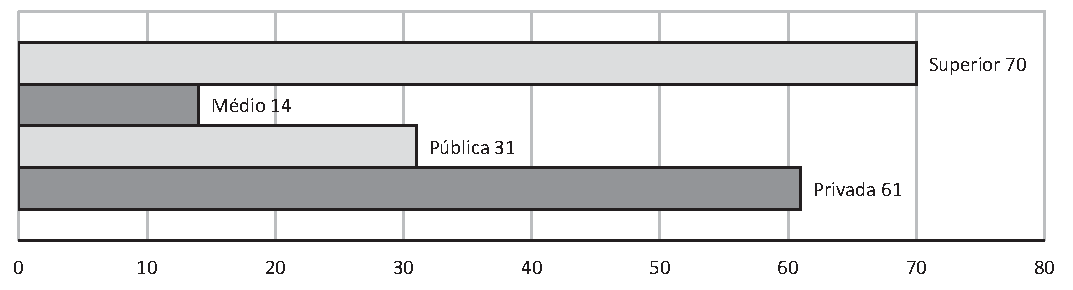
\includegraphics[width=1.0\textwidth]{pdfs/professores/img-grafico-nivel.pdf} 
%\caption{Nível e tipo de escola}
%\label{fig:grafico_nivel} 
%\end{figure}


%\subsection{Modalidade pedagógica e uso de tecnologia em sala de aula}

A modalidade pedagógica mais utilizada pelos professores ainda é a aula expositiva que esteve presente em 79 respostas, seguidas por aulas dialogadas com 60, pesquisas com 61, BPL com 42, visitas com 19 e outros com 8 respostas. A Figura \ref{fig:grafico_modalidade} mostra graficamente os resultados desta questão. 

%As respostas quanto a modalidade pedagógica visa revelar quais as estratégias de ensino mais utilizadas pelos professores, esta informação pode revelar uma relação entre modalidade e tecnologia utiliza em sala de aula.

%A Figura \ref{fig:grafico_modalidade} mostra graficamente os resultados obtidos por esta questão. É importante notar que aulas expositivas ainda é amplamente utilizada com 79 respostas, seguidas por aulas dialogadas com 60, pesquisas com 61, BPL com 42, visitas com 19 e outros com 8 respostas.
 
\begin{figure}[!h]
\centering
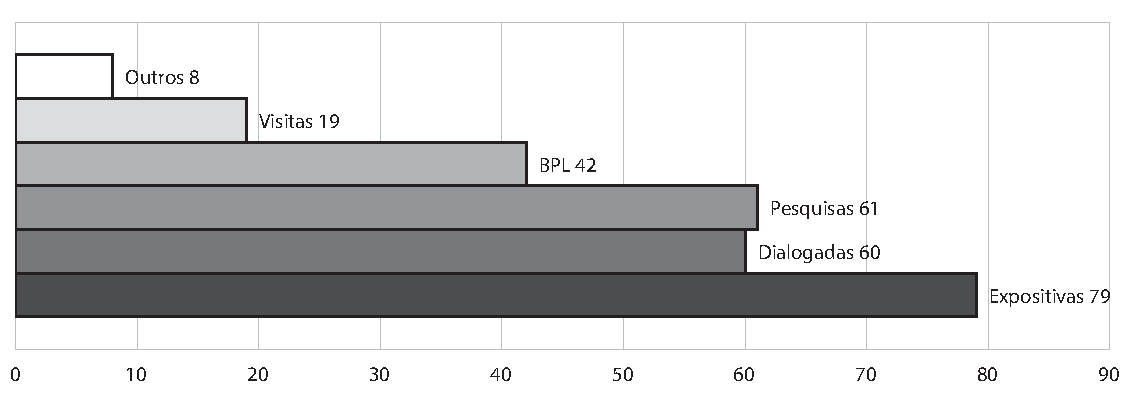
\includegraphics[width=1.0\textwidth]{pdfs/professores/img-grafico-modalidade.pdf} 
\caption{Modalidades pedagógicas}
\label{fig:grafico_modalidade} 
\end{figure}


Já quanto as atividades extra-classe os professores responderam que utilizam muito exercícios, trabalhos de pesquisa e trabalhos práticos, onde os dois primeiros são utilizados por pelo menos 65 dos 81 pesquisados, e o último por 58. 

As atividades extra-classe que poderiam gerar algum tipo de colaboração, como é o caso do fórum de discussões, ainda são pouco utilizadas, sendo a opção de 18 professores. A Figura \ref{fig:grafico_atividades_extra_classe} ilustra graficamente as respostas a esta pergunta.

 
\begin{figure}[!h]
\centering
\includegraphics[width=1.0\textwidth]{pdfs/professores/img-grafico-extra-classe.pdf} 
\caption{Atividades extra-classe}
\label{fig:grafico_atividades_extra_classe} 
\end{figure}


%\subsection{Recursos utilizados}

A pesquisa também abordou questões sobre quais recursos eram mais utilizados em aula pelos professores. As respostas foram bastante coerentes ao tipo de aulas mais utilizadas, sendo recursos mais comumente utilizados em aulas expositivas. Neste caso, o datashow/projetor é utilizado por todos os professores que responderam a pesquisa, e o quadro branco/negro por 74 dos 81 professores. O terceiro recurso em uso são os sistemas de apoio como Moodle e Sakai que são utilizados por 40 pesquisados.

A Figura \ref{fig:grafico_recursos} mostra graficamente o total de respostas para cada tipo de recurso.
 
\begin{figure}[!h]
\centering
\includegraphics[width=1.0\textwidth]{pdfs/professores/img-grafico-recursos.pdf} 
\caption{Recursos utilizados}
\label{fig:grafico_recursos} 
\end{figure}

A pesquisa levantou também se as instituições oferecem sistemas para gerenciamento de conteúdo, como por exemplo, Moodle, Blackboard, Sakai, etc. A resposta de 57 professores é que a sua instituições oferecem, 22 deles disseram que a instituição não oferece e 5 deles que a instituição não oferece mas eles usam um por conta própria. 

%A Figura \ref{fig:grafico_sistemas} mostra graficamente estas respostas.

%\begin{figure}[!h]
%\centering
%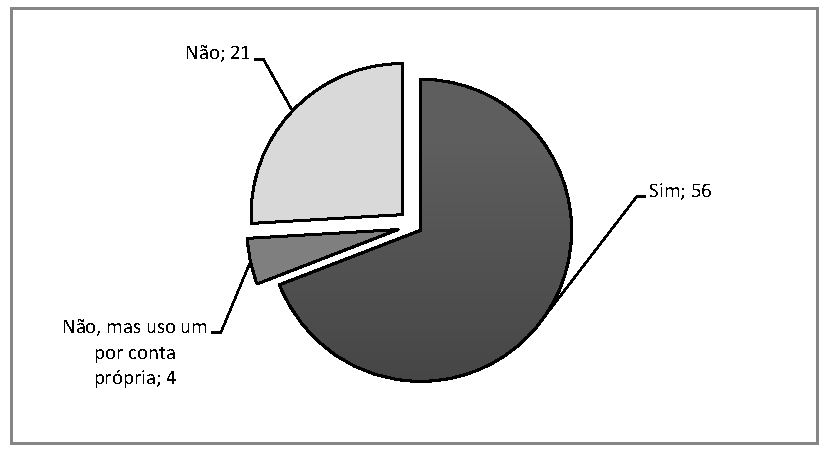
\includegraphics[width=1.0\textwidth]{pdfs/professores/img-grafico-sistemas.pdf} 
%\caption{Sistemas}
%\label{fig:grafico_sistemas} 
%\end{figure}

%\subsection{Retorno dos alunos}

Foi perguntado também se os professores conseguem, de alguma forma, saber a opinião dos alunos sobre as aulas, mesmo sem obter um retorno direto dos alunos. Neste quesito, 45 professores dos 81 pesquisados responderam que conseguem saber deste andamento através do comportamento dos alunos e pelas atividades realizadas em aula. Uma parcela dos professores (18) conseguem também obter esta informação somente através de atividades realizadas em aula, e 16 deles somente através do comportamento dos alunos, e 4 deles não conseguem avaliar.

A Figura \ref{fig:grafico_retorno} mostra graficamente estas respostas dos professores, que 37 pesquisados dizem obter esta informação com muita confiança e 34 com confiança média. Outra informação relevante que foi levantada é que 75 pesquisados gostariam de obter este retorno com mais frequência.

\begin{figure}[!h]
\centering
\includegraphics[width=1.0\textwidth]{pdfs/alunos-professores/pesquisa-retorno-alunos.pdf} 
\caption{Retorno dos alunos}
\label{fig:grafico_retorno} 
\end{figure}

Ainda relacionado ao retorno dos alunos sobre a aula, a pesquisa ainda questionou se os professores percebem ou acham que seus alunos ainda se sentem inibidos em dar algum retorno sobre a aula ou realizar questionamentos. Um pouco mais da metade (43) dos pesquisados acham que algumas vezes sentem seus alunos inibidos, e 18 deles acham que isso acontece muitas vezes. A Figura \ref{fig:grafico_inibicao} mostra graficamente estas respostas.

\begin{figure}[!h]
\centering
\includegraphics[width=1.0\textwidth]{pdfs/alunos-professores/pesquisa-inibicao-alunos.pdf} 
\caption{Inibição dos alunos em dar retorno ou fazer questionamento em aula }
\label{fig:grafico_inibicao} 
\end{figure}


%\subsection{Uso de internet pelos alunos}

A pesquisa buscou também conhecer sobre a utilização de internet pelos alunos tanto dentro quanto fora da sala de aula. Assim sendo, 79 professores acham que seus alunos acessam a internet no dia-a-dia. Foi perguntado também se os professores sabem quantos de seus alunos usam a internet em seus dispositivos móveis durante a aula, sendo que 6 responderam \emph{Todos os alunos}, 23 \emph{Muitos alunos}, e 26 \emph{Alguns alunos}. A Figura \ref{fig:grafico_internet_sala} mostra graficamente os dados completos. Importante notar também que dos professores que responderam que seus alunos usam a internet em sala de aula, 25 deles acham que seus alunos utilizam com finalidade acadêmica e 46 acham que utilizam para fins pessoais.

\begin{figure}[!h]
\centering
\includegraphics[width=1.0\textwidth]{pdfs/alunos-professores/pesquisa-uso-internet-sala.pdf} 
\caption{Uso de internet em sala de aula pelos alunos}
\label{fig:grafico_internet_sala} 
\end{figure}

Foi pesquisado também se os professores gostariam de saber quanto seus alunos estudam em casa e, 72 deles responderam que gostariam de conhecer esta informação, contra 9 que não desejariam.

\section{Análise dos resultados específicos a alunos}

O total de alunos que responderam ao questionário foi de 126, onde a média de idade dos respondentes foi de 24 anos de idade, informação que pode indicar que estes alunos desde a infância e/ou adolescência já possuem contato com tecnologias digitais. Sobre a localização destes alunos 75 são do estado de MG (59,52\%) e 43 (34,13\%) de SP, números justificados por ser os estados de origem dos autores. Sobre o tipo de instituição que cada aluno pertence, 39 (30,7\%) estudam em instituições públicas e 88 (69,3\%) em privadas. Outro fator levantado também foi que 7 alunos (5,5\%) estudam no ensino-médio e 120 (94,5\%) no ensino superior ou pós-graduação.

Os alunos responderam sobre quais modalidades pedagógicas eles aprendem melhor, e pelo ponto de vista dos mesmos, aulas dialogadas é a que mais obtém resultados. A Figura \ref{fig:metodologia_alunos} compara graficamente o número de respostas de cada modalidade.

\begin{figure}[!h]
\centering
\includegraphics[width=1.0\textwidth]{pdfs/alunos-professores/pesquisa-alunos-modalidade-pedagogicas.pdf} 
\caption{Quais metodologias pedagógicas os alunos aprendem mais}
\label{fig:metodologia_alunos} 
\end{figure}

Os alunos responderam também sobre quais recursos o seu professor utiliza em salas de aula. O recurso de quadro negro ou branco e projetor foram as mais marcadas, com 107 e 121 respostas, respectivamente. A Figura \ref{fig:recursos_professores} compara graficamente o número de respostas de cada recurso.

\begin{figure}[!h]
\centering
\includegraphics[width=1.0\textwidth]{pdfs/alunos-professores/pesquisa-alunos-recursos-que-seu-professor.pdf} 
\caption{Quais os recursos seus professores utilizam}
\label{fig:recursos_professores} 
\end{figure}

Já sobre as atividades extra-classe muitos alunos acham que aprendem mais fazendo exercícios práticos, com 81,9\% (104).

Um fator explorado no questionário foi sobre a comunicação entre alunos e professores em sala de aula. Um exemplo deste tipo de informação é relacionada a se os alunos informam seu entendimento sobre as aulas aos professores, ou se os alunos ainda sentem-se inibidos ao realizar questionamentos. Em 17,3\% (22) das respostas dos alunos eles não informam ao professor sobre seu entendimento de aula, em 46,6\% (59) informam somente as vezes e em 36,2\% (46) informam sempre. A justificativa dos alunos para não informarem aos professores sobre o entendimento das aulas, de acordo com algumas justificativas recebidas estão relacionadas a inibição, falta de interesse por parte do aluno, falta de diálogo com os professores ou simplemente porque o aluno não gosta de o fazer. Já as justificativas dos alunos que dão este retorno ao professor o fazem para obter um melhor entendimento da aula e para ajudar ao professor a mensurar seus resultados, como justitificado por estes alunos: ``Por que acho importante o feedback ao professor sobre a abordagem e conteúdos apresentados.'', ``Para que ele saiba que conseguiu atingir sua meta'' e ``Acho necessário que ele entenda como os alunos estão acompanhando o conteúdo''.

Em 66,1\% das respostas, os alunos gostariam de possuir uma forma de opiniar sobre a aula aos professores de forma anônima, e na Figura \ref{fig:grafico_inibido} mostra graficamente o quanto os alunos ainda se sentem inibidos para dar algum retorno ao professor ou realizar questionamentos. Pode-se perceber que uma porcentagem pequena (22\%) nunca sente-se inibido.

\begin{figure}[!h]
\centering
\includegraphics[width=1.0\textwidth]{pdfs/alunos-professores/pesquisa-inibicao-alunos.pdf} 
\caption{Inibição dos alunos ao fazer questionamentos ou dar um retorno sobre a aula aos professores}
\label{fig:grafico_inibido} 
\end{figure}

Sobre o uso de internet em sala de aula, 33,9\% (43) dos alunos responderam que utilizam quase sempre, e 47,2\% (60) responderam que utilizam quando o professor permite. O interessante desse levantamento é a quantidade de alunos que disseram que utilizam internet em sala de aula, mostrando o quanto a mesma já está presente no ambiente escolar seja com a aprovação do professor ou não. Dos alunos que disseram que utilizam internet em sala de aula, 90,3\% (93) disseram que utilizam para fins acadêmicos e 65\% (67) para fins pessoais, lembrando que esta questão não era exclusiva e portanto o aluno poderia marcar que faz ambos os usos. Na Figura \ref{fig:grafico_uso_internet_alunos_sala} compara-se graficamente a utilização de internet por alunos na sala de aula.

\begin{figure}[!h]
\centering
\includegraphics[width=1.0\textwidth]{pdfs/alunos-professores/pesquisa-alunos-uso-internet-sala.pdf} 
\caption{Utilização de internet em sala de aula pelos alunos}
\label{fig:grafico_uso_internet_alunos_sala} 
\end{figure}



%- recursos computacionais que usa
%- tempo de uso de internet
%- quais tipos de aula vc acha que aprende melhor
%- extra-classe
%- seu prof utiliza nas disciplinas
%- sua instituicao oferece sistemas
%- você informa seu professor sobre o seu entendimento
%- vc gostaria de opinar de forma anonima
%- vc se sente inibido
%- vc faz uso de internet em sala de aula
%- tipo de uso (academico / pessoais)
%- 

\section{Avaliação do uso de internet e tecnologias por professores e alunos}

A pesquisa contém uma seção de quesitonamentos para conhecer um pouco do perfil de alunos e professores em relação ao uso de tecnologia e internet no seu dia-a-dia e em sala de aula. 

Na análise de tipos de aplicativos e ferramentas que alunos e professores utilizam, um fato interessante é que os alunos possuem uma tendência a utilizar recursos computacionais que exigem um pouco mais de conhecimento, como por exemplo, Editores Gráficos são utilizados por 104 de 126 alunos e Planilha Eletrônica são utilizadas por 117 de 126 alunos. E recursos como Internet, Apresentações e Editor de Textos praticamente utilizados por todos os alunos. O fato dos alunos possuírem uma maior desenvoltura com tecnologia beneficia a utilização e a integração de tecnologia em sala de aula.

Já analisando a mesma questão para os professores, os recursos mais utilizados são Internet, Apresentações e Editor de Textos, o que pode indicar que muitos professores ainda utilizam apenas aplicativos mais básicos e poderiam enfrentar dificuldades ou não estarem motivados a aplicar tecnologia em sala de aula. A Figura \ref{fig:grafico_recursos} mostra graficamente os valores relacionados aos recursos tecnológicos e seus usos entre alunos e professores.

\begin{figure}[!h]
\centering
\caption{Recursos computacionais utilizados por alunos e professores}
\includegraphics[width=1.0\textwidth]{pdfs/alunos-professores/recursos-computacionais.pdf} 
\label{fig:grafico_recursos} 
\end{figure}

O uso de internet foi outra informação levantada através do questionário. Nesse item, foi levantado que 67,90\% dos professores e 76\% dos alunos utilizam mais que 20 horas internet por semana. Já o uso de até 5 horas semanais representou 3,17\% e 3,70\%, para alunos e professores, respectivamente. Estes números evidenciam que tanto alunos como professores estão cada vez mais conectados e que passam um boa quantidade de horas semanais utilizando internet. A Figura \ref{fig:grafico_uso_internet} mostra graficamente o uso de cada faixa de horas para alunos e professores.

\begin{figure}[!h]
\centering
\caption{Quantidade de horas que alunos e professores utilizam por semana}
\includegraphics[width=1.0\textwidth]{pdfs/alunos-professores/uso-internet.pdf} 
\label{fig:grafico_uso_internet} 
\end{figure}



\section{Opinião dos professores e alunos quanto a uma futura ferramenta}

A pesquisa em sua segunda parte tem como objetivo saber a opinião dos alunos e professores em relação a uma futura ferramenta a ser utilizada dentro e fora de sala de aula. O primeiro questionamento foi exatamente saber o quão importante é esta ferramenta ser multiplataforma. Mais de metade (62) dos professores consideraram esta característica como muito importante (39) ou de total importância (23), já os alunos também definiram em grande parte como importante, sendo 58 como muito importante e 45 como de total importância . A Figura \ref{fig:grafico_multiplataforma} compara as respostas de alunos e professores relativamente. 

\begin{figure}[!h]
\centering
\caption{Importância da ferramenta ser multiplataforma, comparação entre as respostas de professores e alunos}
\includegraphics[width=1.0\textwidth]{pdfs/alunos-professores/funcionalidades-multiplataforma2.pdf} 
\label{fig:grafico_multiplataforma} 
\end{figure}

Sobre a possível funcionalidade onde os alunos pudessem visualizar o conteúdo de aula do professor em tempo-real grande parte dos professores e alunos definiram como muito importante ou de total importância. A Figura \ref{fig:grafico_visualizar}.

\begin{figure}[!h]
\centering
\caption{Importância da ferramenta permitir que os alunos visualizem o conteúdo em tempo-real, comparação entre as respostas de professores e alunos}
\includegraphics[width=1.0\textwidth]{pdfs/alunos-professores/funcionalidades-visualizar-conteudo.pdf} 
\label{fig:grafico_visualizar} 
\end{figure}

Outra funcionalidade questionada na pesquisa é relacionada a possibilidade de alunos e professores adicionarem informações sobre o material de aula. Sobre esta característica em um futuro sistema a ser utilizado na educação, alunos e professores também marcaram como de total importância ou muito importante, somando 72,84\% e 65,88\% para professores e alunos, respectivamente, indicando assim uma funcionalidade muito relevante ao escopo educacional. A Figura \ref{fig:grafico_anotacoes} compara graficamente as respostas de alunos e professores. 

\begin{figure}[!h]
\centering
\caption{Importância da ferramenta permitir que os alunos anotem sobre o conteúdo, comparação entre as respostas de professores e alunos}
\includegraphics[width=1.0\textwidth]{pdfs/alunos-professores/funcionalidades-anotacoes.pdf} 
\label{fig:grafico_anotacoes} 
\end{figure}


Ainda sobre esta funcionalidade foi questionado a opção destas informações adicionadas ao material de aula poderem ser compartilhadas opcionalmente entre os demais usuários, sendo que também grande parte das respostas marcaram como de total importância ou muito importante, somando 67,9\% e 62,7\% para professores e alunos, respectivamente. A Figura \ref{fig:grafico_compartilhar_anotacoes} compara graficamente estas respostas.


\begin{figure}[!h]
\centering
\caption{Importância da ferramenta ser multiplataforma, comparação entre as respostas de professores e alunos}
\includegraphics[width=1.0\textwidth]{pdfs/alunos-professores/funcionalidades-compar-anotacoes.pdf} 
\label{fig:grafico_compartilhar_anotacoes} 
\end{figure}

A funcionalidade da ferramenta permitir o retorno anônimo do aluno é uma nova forma de comunicação possível entre alunos e professores, e pode ser utilizada como um termômetro em sala de aula permitindo ao professor possuir mais um indicador de motivação e/ou satisfação dos alunos, podendo adequar sua aula a medida que a mesma está acontecendo ou analisando estes dados posteriormente. Sobre esta funcionalidade, também grande parte das respostas de alunos e professores consideram-a como importante, somando 77,78\% e 51,58\%, respectivamente, como de total importância e muito importante. A Figura \ref{fig:grafico_retorno} mostra graficamente estas respostas.

\begin{figure}[!h]
\centering
\caption{Importância da ferramenta permitir um retorno anônimo dos alunos aos professores sobre as aulas (respostas de professores e alunos)}
\includegraphics[width=1.0\textwidth]{pdfs/alunos-professores/funcionalidades-retorno.pdf} 
\label{fig:grafico_retorno} 
\end{figure}


% figura 11
%\begin{figure}[!h]
%\centering
%\caption{Importância da ferramenta ser multiplataforma, comparação entre as respostas de professores e alunos}
%\includegraphics[width=1.0\textwidth]{pesquisa/multiplataforma-relativo.pdf} 
%\label{fig:grafico_multiplataforma} 
%\end{figure}

%\begin{figure}[!h]
%\centering
%\caption{Importância da ferramenta ser multiplataforma respostas de alunos e professores acumuladas}
%\includegraphics[width=1.0\textwidth]{pesquisa/multiplataforma-acumulativo.pdf} 
%\label{fig:grafico_multiplataforma_acumulativo} 
%\end{figure}


%Outra funcionalidade explorada na pesquisa, supõe um sistema que possibilite que o professor disponibilize materiais aos alunos, e os mesmos possam visualizar em tempo real e após a aula. Quanto à relevância desta funcionalidade, 21 professores responderam ser de total importância, 43 como muito importante e 14 de importância média. A Figura \ref{fig:grafico_conteudos} mostra graficamente estas respostas.

%\begin{figure}[!h]
%\centering
%\includegraphics[width=1.0\textwidth]{pdfs/alunos-professores/funcionalidades-visualizar-conteudo.pdf} 
%\caption{Importância da ferramenta permitir distribuir o material de aula em tempo real}
%\label{fig:grafico_conteudos} 
%\end{figure}

%Sobre a possibilidade de receber, através de uma ferramenta, o retorno em tempo real de quanto os alunos julgam estar entendendo do conteúdo foi qualificada como de total importância por 29 professores, muito importante por 35 e de importância média por 13. E 7 professores consideram pouco importante esta funcionalidade. A Figura \ref{fig:grafico_ferramenta_retorno} mostra graficamente estas respostas.

%\begin{figure}[!h]
%\centering
%\includegraphics[width=1.0\textwidth]{pdfs/alunos-professores/funcionalidades-retorno.pdf} 
%\caption{Importância da ferramenta permitir um retorno em tempo real sobre a aula}
%\label{fig:grafico_ferramenta_retorno} 
%\end{figure}

%Ainda sobre a possibilidade de receber retorno dos alunos, foi perguntado também sobre a relevância de manter o histórico destes retornos. Sendo que 22 professores marcaram como total importância, 40 como muito importante, 17 com importância média, 2 como pouco importante e 1 como nada importante.
%A última funcionalidade que teve sua importância investigada é a possibilidade dos alunos fazerem anotações diretamente sobre os materiais de aula que os professores disponibilizarem. Sobre esta funcionalidade, 24 marcaram como sendo de total importância, 34 como muito importante, 19 com importância média e 4 como pouco importante. A Figura \ref{fig:grafico_anotacao} mostra graficamente estas respostas.

%\begin{figure}[!h]
%\centering
%\includegraphics[width=1.0\textwidth]{pdfs/alunos-professores/funcionalidades-anotacoes.pdf} 
%\caption{Importância da ferramenta permitir que alunos façam anotações sobre os materiais de aula}
%\label{fig:grafico_anotacao} 
%\end{figure}


%Também foi da importância de permitir que estas notas sejam compartilhadas. Neste caso, 18 professores disseram ser de total importância, 36 como muito importante, 23 com importância média, 3 como pouco importante e 1 como nada importante.

\section{Considerações}

A pesquisa possibilitou conhecer um pouco mais sobre uma parte do público deste trabalho. Também permitiu conhecer os recursos utilizados e perceber que estes são diretamente ligados ao tipo de metodologia pedagógica mais amplamente utilizado.

Alguns professores fizeram considerações interessantes sobre uma ferramenta com as características propostas. Como por exemplo, um professor considera a possibilidade de permitir ao aluno pesquisar na internet durante a aula de extrema importância para demonstrar sua capacidade de raciocínio e consequentemente seu interesse na aula e no tema. Outro professor, acha que ao oferecer uma ferramenta como esta, a grande maioria dos alunos passariam a utilizar internet em aula com a finalidade acadêmica deixando assim de utilizar para fins pessoais.

Os resultados desta pesquisa serão também utilizados para nortear quais e como as funcionalidades da ferramenta deverão ser projetas e desenvolvidas, sendo um fator muito importante ao levantamento de requisitos descrito no Capítulo \ref{cap:mindboard}.


\chapter{O sistema Mindboard}
\label{cap:mindboard}

Este capítulo tem como objetivo detalhar o projeto e desenvolvimento do sistema Mindboard. O desenvolvimento seguirá o processo unificado customizado de forma similar à proposta por \citeonline{joao_pu}.

\section{O Processo Unificado e suas customizações}

O Processo Unificado foi inicialmente discutido por \citeonline{jacob99} em sua busca por um processo de software guiado por casos de uso, centrado na arquitetura, iterativo e incremental. Segundo \citeonline{pressman06} o Processo Unificado é uma tentativa de apoiar-se nos melhores recursos e características de modelos convencionais de processo de desenvolvimento de software reforçando pontos de desenvolvimento ágil.

\citeonline{pressman06} descreve um arcabouço de um processo genérico, onde o mesmo é composto pelas fases de Comunicação, Planejamento, Modelagem, Construção e Implantação. Na fase de Comunicação acontece toda a troca de informações com os interessados no projeto e clientes, e inclui o levantamento de requisitos e atividades relacionadas. A fase de Planejamento, define e estabelece as tarefas futuras a serem desenvolvidas, juntamente com os riscos, recursos necessários, produtos de trabalhos que serão gerados e um cronograma do trabalho. A fase de Modelagem é a atividade onde são desenvolvidas modelos que facilitam o entendimento pelos desenvolvedores e cliente dos requisitos e do projeto que irá satisfazer os mesmos. Na fase de Construção são desenvolvidas as atividades de geração de códigos fonte e de testá-los. E a fase de Implantação, que é a fase final, o software completo ou uma atualização do mesmo é entregue ao cliente \cite{pressman06}. A Figura \ref{fig:processo_unificado} ilustra a ordem em que estas fases acontecem.

O Processo Unificado é composto por ciclos que passam por atividades contidas nas fases genéricas de um processo descritas anteriormente por \citeonline{pressman06}, porém de uma maneira iterativa e incremental. As fases no Processo Unificado são nomeados de forma diferente, sendo elas a Concepção, Elaboração, Construção, Transição e Produção.

A fase de Concepção abrange as atividades das fases de Comunicação e Planejamento do processo genérico descrito anteriormente. Durante a Concepção acontecem as atividades de comunicação com o cliente e usuários finais, é realizada a descrição dos requisitos, uma arquitetura é proposta, e um plano de trabalho para este ciclo/incremento é criado. Nesta fase é comumente utilizado diagramas que facilitem o entendimento e comunicação entre os interessados no projeto, como Diagramas de Casos de Uso e Diagramas de Classes \cite{pressman06}. Nesta fase deve-se também avaliar o contexto onde o projeto será inserido verificando seu impacto e retorno. Caso o retorno seja mínimo ou não valha a pena, pode ser cancelado após esta fase \cite{sommerville10}.

Após a Concepção, a iteração passa para a fase de Elaboração incluindo as atividades das fases de Planejamento e Modelagem do processo genérico. A Elaboração expande os Casos de Usos e Diagramas de Classes gerados na fase anterior, permitindo uma visão mais específica e refinada sobre os requisitos \cite{pressman06}. O objetivo principal desta fase é desenvolver uma visão sólida do domínio, estabelecer um arcabouço arquitetural, definir um planejamento e identificar os principais riscos \cite{sommerville10}.

A fase de Construção é idêntica a do processo genérico \cite{pressman06}, envolvendo projetar, programar e testar o sistema, incluindo o desenvolvimento de testes unitários. Partes do sistema desenvolvidas em paralelo são integradas nesta fase. Ao final desta fase, deve-se gerar uma versão funcional do software e sua documentação relacionada pronta para entrega aos interessados \cite{sommerville10}. 

Já na fase de Transição acontece a mudança do sistema/conjunto de funcionalidades do estado de desenvolvimento para produção \cite{sommerville10}. Quando relacionado ao processo genérico, esta fase abrange os últimos estágios de Construção e a primeira da Implantação, e nesta fase o cliente e usuários finais possuem contato com uma versão beta do software e é possível que eles dêem retorno sobre o mesmo  \cite{pressman06}.

A Figura \ref{fig:processo_unificado} ilustra as fases do Processo Unificado e seus relacionamentos ao processo genérico definido por \citeonline{pressman06}. Os itens delimitados por linhas pontilhadas são pertencentes ao Processo Unificado, e as de linhas contínuas, pertencem ao processo genérico de software.

\begin{figure}[!h]
\centering
\caption{As fases de um processo genérico relacionadas com as fases do Processo Unificado}
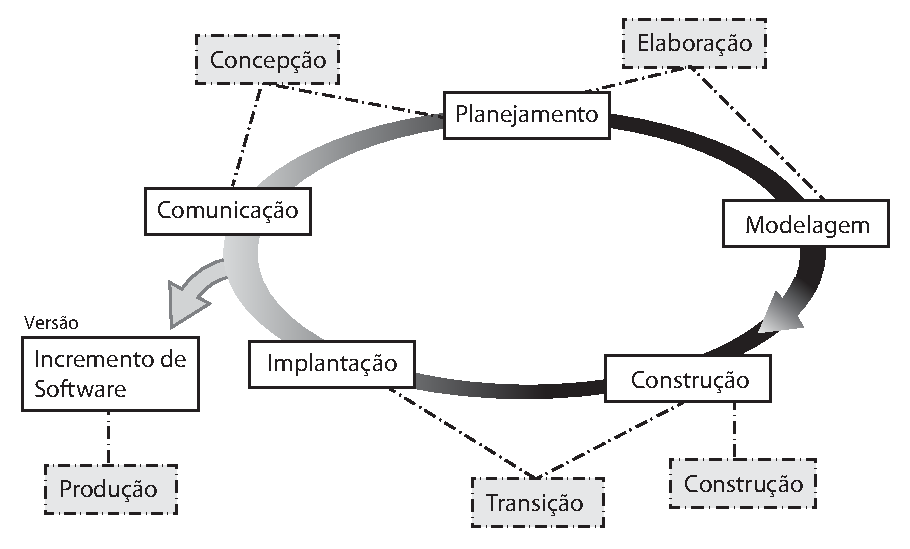
\includegraphics{pdfs/img-processo-unificado.pdf}
\source{\citeonline{pressman06}}
\label{fig:processo_unificado} 
\end{figure}

O Processo Unificado permite escolher, de acordo com as características de cada projeto, a forma como as mesmas são percorridas, ou seja, são iteradas. As iterações podem acontecer de duas formas: a) cada fase pode ser conduzida de forma iterativa com os resultados desenvolvidos de forma incremental; b) todo o conjunto de fases podem ser conduzidas de forma incremental \cite{sommerville10}.

Na Figura \ref{fig:processo_unificado_iteracoes} as setas menores indicam a possibilidade de seu comportamento incremental nas atividades daquela fase. Já a seta maior, indica o cenário onde todas as fases são percorridas incrementalmente.

\begin{figure}[!h]
\centering
\caption{Formas de iteração do Processo Unificado}
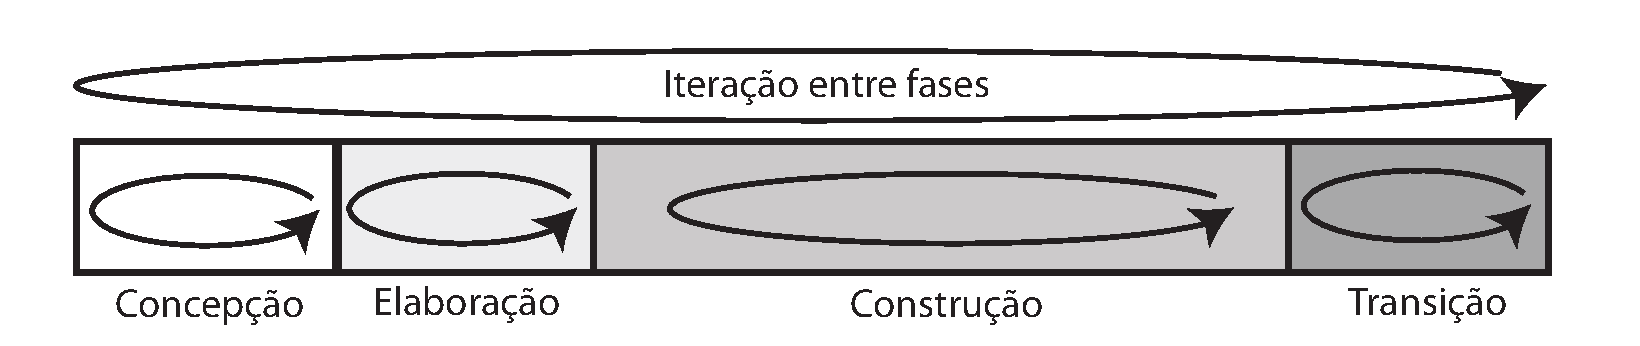
\includegraphics[width=1.0\textwidth]{pdfs/img-processo-unificado-fases.pdf}
\source{\citeonline{sommerville10}}
\label{fig:processo_unificado_iteracoes} 
\end{figure}

\section{Customizações do Processo Unificado}

Neste trabalho, para o desenvolvimento do sistema será utilizado o Processo Unificado com as customizações propostas por \citeonline{joao_pu}, que propõe algumas simplificações no Processo Unificado convencional possíveis pelo baixo risco financeiro do projeto, pela pequena escala envolvendo um único desenvolvedor e para a redução do número de artefatos artefatos gerados.

De acordo com \citeonline{smith:2001} em projetos com estas características as fases de Concepção e Elaboração podem ser reduzidas a uma rápida análise de viabilidade e com a definição de um cronograma de alto nível para as atividades do trabalho, que é refinado em cada etapa.

Este projeto terá documentado exclusivamente a fase de Construção, pois dentro desta fase, segundo \citeonline{jacob99}, pode ser absorvida as atividades de requerimento, projeto e implantação em projetos de pequeno porte, e portanto, não precisa ser realizada explicitamente.

A etapa de projeto é bastante estendida em projetos de pesquisa pois inclui o desenvolvimento de, experimentação com, protótipos. A última alteração no Processo Unificado proposto é em relação aos artefatos gerados. Embora tenha sido dividido em várias iterações, serão mantidos apenas as versões integradas dos mesmos.

Outra simplificação proposta por \citeonline{joao_pu} está relacionada com as iterações do processo. O desenvolvimento deste projeto foi dividido em 4 iterações incrementais. As etapas de cada iteração serão descritas de uma única vez e serão mantidos somente os artefatos gerados já resultantes de todas as iterações realizadas até cada momento.


\section{Iterações}

As iterações no Processo Unificado fundamentalmente seguem a ideia que problemas menores são mais fáceis de resolver que problemas maiores \cite{arlow:2002}. Assim, o Processo Unificado divide um projeto em ``projetos menores'' que são mais fáceis de gerenciar e desenvolver. Cada ``projeto menor'' é uma iteração \cite{arlow:2002}, e o grande ponto chave que cada iteração passa pelas mesmas fases descritas anteriormente.

%O Processo Unificado é conhecido principalmente por se tratar de uma metodologia em que cada uma de suas fases é composta por uma ou mais iterações. Como descrito anteriormente, as fases de concepção e elaboração foram feitas objetivamente em uma iteração, porém a fase de construção é composta pelas iterações descritas a seguir:

O projeto e desenvolvimento do sistema Mindboard aconteceu em quatro iterações. Na primeira iteração foi focada em determinar a arquitetura mais adequada aos requisitos de escalabilidade e extensibilidade. Nesta fase também foi estruturada como será realizada a comunicação entre os participantes de uma sessão, desde a arquitetura bem como o protocolo utilizado. Foram codificadas nesta fase provas de conceitos para que estas funcionalidades fossem experimentadas.

A segunda iteração é focada em desenvolver as funcionalidades de envio de apresentações de slides, permitindo a anotação colaborativa sobre os mesmos, funcionalidade presente em alguns dos trabalhos analisados na revisão da literatura mas não disponível em nenhum dos sistemas comerciais. Nesta interação também são desenvolvidas a geração de enquetes e o recebimento de retorno dos alunos sobre o andamento das aulas e serão projetadas e codificadas as políticas de visibilidade de informação, de modo que cada usuário que contribuir com informações poderá definir quem poderá visualizar a mesma.

Na terceira iteração, a interface é desenvolvida com o objetivo principal de obter uma interface responsiva que se adapta em dispositivos com telas de tamanhos distintos. Nesta iteração todos os dados e informações geradas e trocadas durante uma sessão terão sua persistência garantida através do uso de um banco de dados.

Já na quarta e última iteração, foi desenvolvida a funcionalidade de possibilitar rever uma sessão, e também toda colaboração assíncrona da ferramenta. Foi adicionada também a funcionalidade de compartilhamento de código-fonte em tempo-real, e o projeto foi disponibilizado para a realização do experimento prático.

Como relatado anteriormente, os artefatos que serão apresentados neste capítulo são o resultado de todas iterações executadas, e não as versões parciais desenvolvidas em cada uma delas.

\section{Captura de requisitos}

Os requisitos funcionais descrevem as funcionalidades que se espera que o sistema disponibilize, de uma forma completa e consistente. É aquilo que o usuário espera que o sistema ofereça, atendendo aos propósitos para qual o sistema está sendo desenvolvido \cite{padua05}.

Neste projeto os requisitos funcionais foram priorizados, adotando as seguintes denominações: essencial, importante e desejável. A Tabela \ref{tab:prioridade_req} descreve o significado de cada uma delas.

\bgroup
\def\arraystretch{1.5} % 1 is the default, change whatever you need
\begin{table}[h]{} % t - top of page - h - here - b - bottom
\caption{Prioridade dos requisitos}
\centering
\begin{tabular}{ | p{3cm} | p{10cm}| } \hline
\textbf{Tipo} & \textbf{Descrição} \\ \hline
Essencial & É o requisito sem o qual o sistema não entra em funcionamento. Requisitos essenciais são requisitos imprescindíveis, que têm que ser implementados.  \\ \hline
Importante  & É o requisito o qual o sistema entra em funcionamento, mas de forma não satisfatória. Requisitos importantes devem ser implementados, mas, se não forem, o sistema pode ser implantado e usado mesmo assim, por exemplo, sendo usado ainda durante o desenvolvimento, fornecendo valor mesmo antes do término do projeto.  \\ \hline
Desejável  & É o requisito que não compromete as funcionalidades básicas do sistema, isto é, o sistema pode funcionar de forma satisfatória sem ele. Requisitos desejáveis são requisitos que podem ser deixados para versões posteriores do sistema caso não haja tempo hábil para implementá-los  \\ \hline
\end{tabular}
\label{tab:prioridade_req}
\end{table}
\egroup

Os requisitos funcionais da ferramenta Mindboard foram motivados pelas funcionalidades encontradas em ferramentas acadêmicas e de mercado através das revisões exploratórias descritas no Capítulo \ref{chap:revisao}, pelas pesquisas conduzidas com professores e alunos do ensino médio e superior em que foi questionada a relevância da presença de determinadas funcionalidades em uma ferramenta multiplataforma para uso dentro e fora de sala de aula. A metodologia utilizada nestas pesquisas foram descritas na Seção \ref{sec:metodologia_professores} e \ref{sec:metodologia_alunos}, e seus resultados encontram-se na Seção \ref{chap:pesquisa_prof} e \ref{chap:pesquisa_prof}, respectivamente. 

%Já os requisitos funcionais para a ferramenta Mindboard são descritos em forma de casos de uso simplificados  \ref{chap:requisitos}.

A publicação de \citeonline{pusnik_investigation_2010}  encontrada através da revisão sistemática mostra a relevância em um sistema de ensino a distância de algumas funcionalidades. Nesta pesquisa, a colaboração entre os alunos é citada como muito importante por 31,5\% e como importante para 43,8\% dos entrevistados. A comunicação com outros alunos também é relacionada como muito importante por 27,7\% e como importante por 42,6\% dos entrevistados. A Tabela \ref{tab:importancia} mostra os resultados completos desta pesquisa. 

Acredita-se que as características levantadas como relevantes em sistemas de ensino a distância também são relevantes ao ensino presencial, tanto para uso dentro como fora de sala de aula, uma vez que a comunicação e colaboração estão cada vez mais presentes em serviços online, e pela própria necessidade das gerações atuais em comunicar-se.

Os requisitos funcionais e não funcionais da ferramenta Mindboard são listadas e descritas no Apêndice \ref{cap:requisitos_f_nf}.


\subsection{Descrição dos atores}

Em um sistema, todos os elementos externos que de alguma forma interajam com o software é chamado de ator. Cada ator desempenha um papel no qual ele utiliza ou interage com os serviços e funções do sistema \cite{guedes:2009}. Para a ferramenta Mindboard, os atores e seus devidos papéis são descritos a seguir.


\textbf{Ator 1 - Usuário}

Todos os usuários previamente cadastrados na ferramenta podem identificar-se no sistema através de um nome de usuário e senha.

\textbf{Ator 2 - Professor}

Usuários do tipo professor podem criar, gerenciar e conduzir sessões. Usuários Professores podem também gerenciar os usuários que podem acessar uma sessão.

\textbf{Ator 3 - Aluno}

Usuários do tipo professor podem criar, gerenciar e conduzir sessões. Usuários Professores podem também gerenciar os usuários que podem acessar uma sessão.

\textbf{Ator 4 - Outro sistema}

Outros sistemas podem interagir com o Mindboard para o gerenciamento de sessões, além de identificar e autenticar usuários.

\subsection{Diagramas de casos de uso}

Os diagramas de caso de uso visam exibir de uma maneira gráfica e rápida os casos de uso da ferramenta projetada. Para a ferramenta Mindboard, os diagramas de casos de uso foram agrupados de acordo com o tipo de usuário que a está utilizando. 

A Figura \ref{fig:use_case1} mostra o caso de uso de identificação de usuários. Todos os usuários deverão executar estes casos de uso antes de utilizar a ferramenta. No caso do ator ser outro sistema, a identificação do usuário bem como as credenciais de acesso são concedidas através de uma interface específica a integrações.
 
\begin{figure}[!h]
\centering
\includegraphics[width=1.0\textwidth]{pdfs/img-use-case1.pdf} 
\caption{Diagrama de casos de uso - identificação e acesso a ferramenta}
\label{fig:use_case1} 
\end{figure}

Os casos de uso da Figura \ref{fig:use_case1} mostram o acesso de um usuário que está utilizando a ferramenta como professor. Nela o mesmo pode gerenciar sessões, e gerar todas as informações que são distribuídas a todos os demais usuários.
 

\begin{figure}[!h]
\centering
\includegraphics[width=1.0\textwidth]{pdfs/img-use-case2.pdf} 
\caption{Diagrama de casos de uso - acesso como professor}
\label{fig:use_case2} 
\end{figure}

A Figura \ref{fig:use_case3} mostra os casos de uso relacionados ao ator aluno. É formado por casos de uso que permitem ao usuário visualizar as informações geradas pelo professor e interagir através de perguntas e do compartilhamento das próprias anotações.

 
\begin{figure}[!h]
\centering
\includegraphics[width=1.0\textwidth]{pdfs/img-use-case3.pdf} 
\caption{Diagrama de casos de uso - acesso como aluno}
\label{fig:use_case3} 
\end{figure}

\subsection{Visão de dados}

O diagrama de classes permite a visualização das classes utilizadas pelo sistema e como estas relacionam, permitindo assim uma visão estática de como os dados utilizados na ferramenta são persistidos. O diagrama de classe do projeto é mostrado na Figura \ref{fig:class_diagram}.


\begin{figure}[!h]
\centering
\includegraphics[width=1.0\textwidth]{pdfs/img-class-diagram.pdf} 
\caption{Diagrama de classes}
\label{fig:class_diagram} 
\end{figure}

A classe Usuário é abstrata e portanto só pode ser instanciada pela suas sub-classes Aluno e Professor. Estas 3 classes que serão utilizadas para representar os dados dos usuários do sistema. A classe Sessão é um periodo de utilização da ferramenta, ela pode ser criada por um Professor ou por um Outro Sistema através da interface de integração.

A classe Evento é relacionada a todo tipo de ação ou atividade realizada dentro de uma sessão. Por exemplo, uma anotação é um evento. Ela possui um auto-relacionamento, pois em determinadas situações como em dúvidas,  pode estar relacionado a resposta da mesma.

A classe Módulo é responsável pelos dados de todos os módulos da ferramenta. Esta classe e as já descritas acima deverã sofrer alterações até a finalização do projeto para que possa atender a todos os requisitos do projeto. 

\iffalse
\subsection{Padrão de projetos MVC - \emph{model-view-controller}}

No desenvolvimento da ferramenta Mindboard será utilizado o padrão de projeto MVC. Este padrão é definido como um padrão em camadas \cite{pressman} que divide o código em 3 partes, e também define como é a comunicação entre elas.

Ao usuário fazer uma requisição na ferramenta, a mesma é mapeada a um \emph{controller}. O \emph{controller} utiliza o \emph{model} ou os \emph{models} responsáveis por realizar a operação em questão e direciona ao \emph{view} que exibirá a interface de forma apropriada \cite{mvc}. A Figura \ref{fig:mvc} mostra este processo em uma ferramenta web.

\fi



\subsection{Tecnologias}
\label{sec:tecnologias}

Os requisitos não funcionais da ferramenta Mindboard sugerem que a mesma possua uma arquitetura que possa ser escalável. Para atingir este objetivo foram pesquisados formas de disposição de servidores que permitissem a adição de recursos computacionais de forma simples. Foram encontrados alguns estudos de caso e relatos em ferramentas comerciais que possuem um grande número de usuários e como a arquitetura pode ser escalável Sendo assim, a arquitetura proposta para a ferramenta Mindboard foi baseada em relatos e estudos de caso de das ferramentas Box.com \cite{boxcom}, Trello \cite{trello} e Boo-Box \cite{boobox}. A Figura \ref{fig:arquitetura} mostra esta arquitetura.

\begin{figure}[!h]
\centering
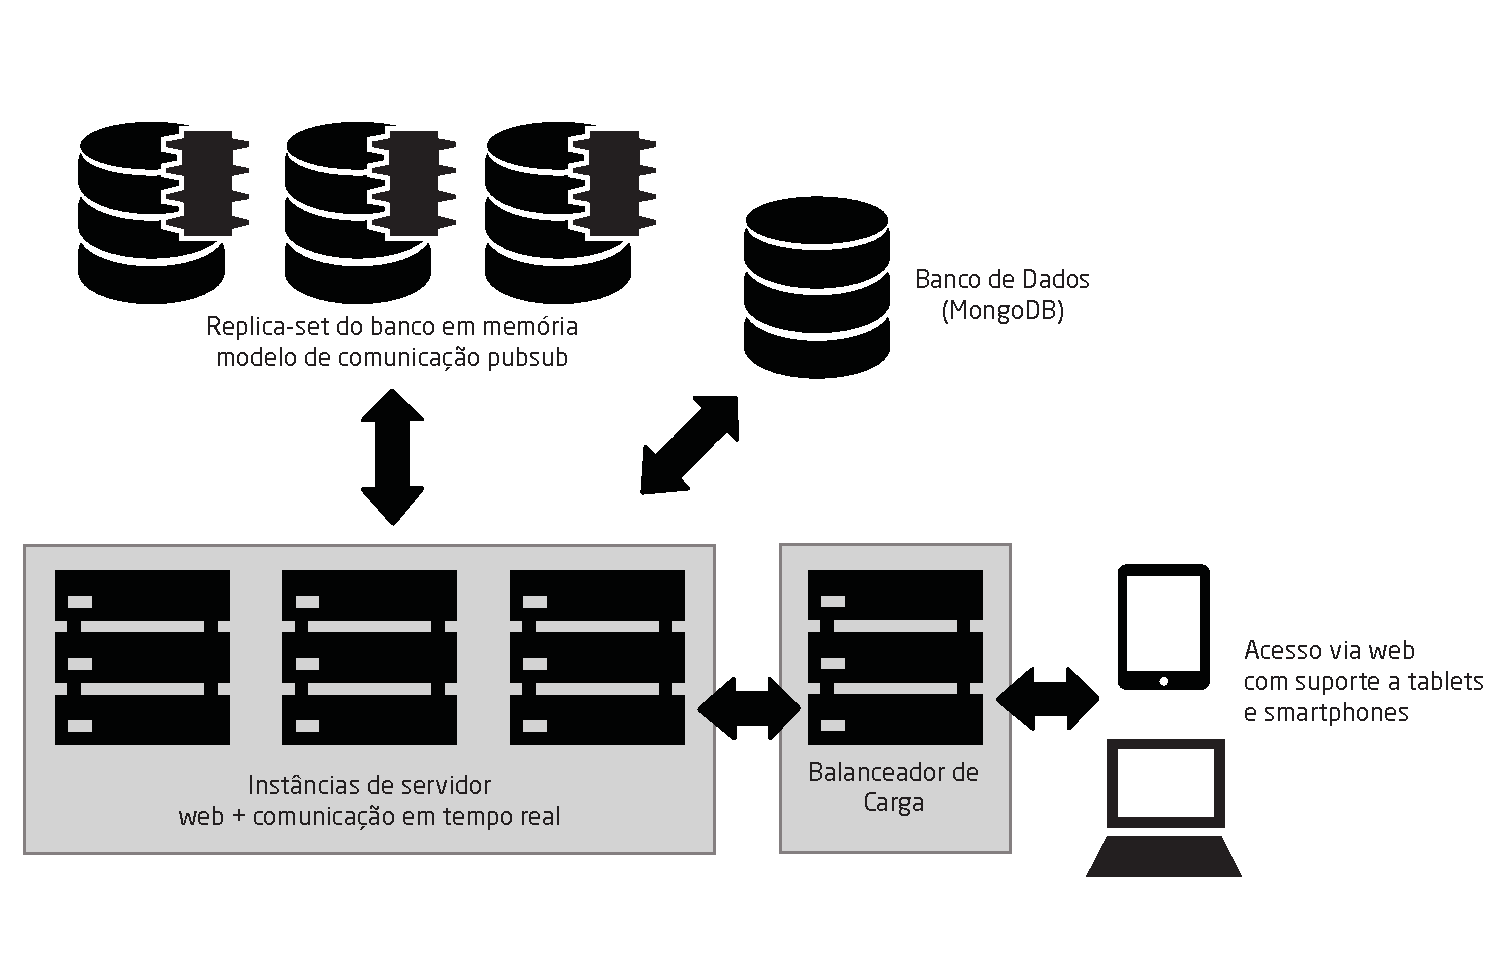
\includegraphics[width=1.0\textwidth]{pdfs/img-arquitetura-lb.pdf} 
\caption{Arquitetura de servidores do Mindboard}
\label{fig:arquitetura} 
\end{figure}

O balanceador de carga é composto por um ou mais servidores que recebem as requisições dos usuários e as redistribui em servidores de aplicação. Durante esta redistribuição o balanceador de carga tenta manter a mesma carga em cada um dos servidores de aplicação.

A camada de servidores de aplicação é responsável por receber as requisições do balanceador de carga e processar de forma completa a requisição do usuário. Em algumas situações será necessário ler e persistir dados, neste caso, a aplicação faz esta operação em um dos servidores de banco de dados. A comunicação entre servidores é realizada utilizando o banco em memória.

O banco de dados é configurado como um \emph{replica-set}, ou seja, vários servidores espelhados e que em cada instância da aplicação pode conectar-se e realizar operações. Nesta configuração há a garantia de disponibilidade de dados e também o aumento da performance.

A camada de comunicação entre servidores é composta por instâncias de servidores em memória utilizando o padrão de comunicação \emph{pubsub}. Esta camada é responsável por permitir uma comunicação entre os servidores de forma rápida, pois os dados não são persistidos e são mantidos apenas em memória.


\section{Tecnologias para front-end}
\label{sec:tecnologias_frontend}

O experimento realizado no LInE, conforme descrito na Seção \ref{sec:metodologia_line}, permitiu levantar indícios sobre a utilização de duas possíveis opções de tecnologias para o desenvolvimento da interface gráfica do sistema Mindboard. Estes indícios, juntamente com outras informações de tendência e compatibilidade que serão descritas nessa seção fortaleceram a decisão técnica da escolha do uso de HTML5, Javascript e CSS 3 como tecnologias \emph{front-end} do sistema.

Toda atividade prática no experimento realizado no LInE gerava uma informação de \emph{log} quando era iniciada e exibida corretamente no navegador do usuário. Sempre que o sistema gerenciador de cursos recebia este evento do módulo de aprendizagem era possível identificar que o mesmo foi visualizado pelo aluno. A Tabela \ref{tab:ivprog} mostra o número de visualizações de cada módulo de aprendizagem juntamente com qual tecnologia o mesmo foi construído, e o número de visualizações em cada atividade semanal.

\begin{table}[h]
\begin{tabular}{lrrrr}
\textbf{Curso}                    & \multicolumn{1}{l}{\textbf{\begin{tabular}[c]{@{}l@{}}Semana 1\end{tabular}}} & \multicolumn{1}{l}{\textbf{\begin{tabular}[c]{@{}l@{}}Semana 2\end{tabular}}} & \multicolumn{1}{l}{\textbf{\begin{tabular}[c]{@{}l@{}}Semana 3\end{tabular}}} & \multicolumn{1}{l}{\textbf{\begin{tabular}[c]{@{}l@{}}Semana 4\end{tabular}}} \\
\textbf{G1 (VPL - Java Applet)} & 517                                                                                              & 217                                                                                              & 80                                                                                               & 70                                                                                               \\
\textbf{G2 (iVProg - Java Applet)}  & 1182                                                                                             & 516                                                                                              & 140                                                                                              & 66                                                                                               \\
\textbf{G3 (iVProg - HTML5/CSS3/JS)} & 1343                                                                                             & 1112                                                                                             & 187                                                                                              & 92                                                                                              
\end{tabular}
\caption{Visualizações da atividade}
\label{tab:ivprog}
\end{table}

Importante notar que apesar do número de visualizações reduzir entre a semana 1 e 4 em todos os grupos, avaliando semana a semana, o G3 obteve mais visualizações que os outros grupos, inclusive na semana 2, obteve mais visualizações que a soma dos demais.

Durante o período do curso foram realizados vários atendimento de suporte aos alunos guiando-os a instalar e configurar de forma apropriada suas máquinas para que fosse possível utilizar o VPL e o iVProg versão \emph{Java Applet}, mesmo assim, para alguns alunos este entrave tecnológico representou uma barreira a utilização do curso e ainda há aqueles alunos que simplesmente desistem e não nos avisaram. Um exemplo do que um aluno com problemas enviou ``Eu tive dificuldades (e ainda estou tendo) em realizar os algoritomos em C \emph{(este aluno pertence a G1 e refere-se ao VPL construído em Java Applet)}, diretamente pela ferramente, pois apesar de ter a versão atualizada do Java em minha máquina eu não consigo pois o sistema informa que minhas configurações de segurança estão bloqueando a aplicação. Gostaria de uma ajuda dos Srs. para resolver isso.''. 

A tecnologia \emph{Java Applet} possui um outro problema o qual vem ocorrendo nas últimas versões do navegador Google Chrome. Esse navegador está removendo progressivamente o suporte a tecnologia que permite que o \emph{Java Applet} seja executado \footnote{https://java.com/en/download/faq/chrome.xml}. Assim, como mais de 60\% dos usuários atualmente utilizam esse navegador \footnote{http://www.w3schools.com/browsers/browsers\_stats.asp}, uma grande parcela dos usuários não poderiam utilizar uma ferramenta feita com essa tecnologia.

A tecnologia HTML 5, Javascript e CSS3 possuem algumas funcionalidades que facilitariam o desenvolvimento do sistema. A API de comunicação em tempo-real do HTML5 favorecem a criação de aplicações que comunicam-se constantemente com o servidor. O CSS3 através de seus media-queries permitem que criemos telas responsivas ao tamanho do dispositivo do usuários.





Após a definição da arquitetura, foram definidas quais tecnologias poderiam ser utilizadas em cada uma delas, começando pela interface com o usuário. 


Os requisitos não funcionais da ferramenta Mindboard norteia a utilização de tecnologias para a criação de interfaces que sejam compatíveis com mais de uma plataforma e que possam conter suporte a dispositivos móveis. Sendo assim, após realizada algumas provas de conceito e após o desenvolvimento de ferramentas utilizadas no grupo de pesquisas LiNE, as tecnologias adotadas foram HTML 5, CSS 3 e JavaScript.

A tecnologia HTML 5 aumentou a padronização no desenvolvimento de aplicações web, principalmente focando em padronizar como utilizar interação entre os elementos \cite{html5}. Visualmente, a interface HTML 5 foi formatada utilizando CSS 3, que inclusive permite a criação de interfaces responsivas. Já JavaScript permite manipular o HTML5 e principalmente realizar a comunicação em tempo real com o servidor.

O servidor de aplicação foi desenvolvido em JavaScript principalmente para manter uma mesma linguagem no servidor e no cliente. Por este motivo, foi utilizado o NodeJS para a execução do código no servidor.

A tecnologia NodeJS é um ambiente que possibilita a execução de códigos JavaScript no servidor utilizando a mesma tecnologia por trás do Google Chrome, a engine V8 \cite{nodejs}. Uma característica muito importante presente no NodeJS que é fundamental para sistemas de comunicação em tempo real, é o fato do código ser \emph{non-blocking} para operações de entrada e saída, isso permite obter uma boa estabilidade e performance para sistemas que possuem comunicação em tempo real \cite{nodejs}.

Já os dados serão persistidos utilizando o banco de dados MongoDB. O MongoDB é um banco não relacional orientado a documentos. Sua estrutura é baseada em coleções de documentos que podem conter estruturas diversas, sendo assim, uma forma de armazenamento que não possui um \emph{schema} definido \cite{mongodb}. 

É uma forma de armazenar grandes volumes de dados de forma bastante eficiente, e de acordo com \cite{mongodb} o tempo para inserir grandes quantidades de informação chega a ser 15 vezes inferior que a inserção da mesma quantidade de informações em um banco de dados Oracle. O tempo para a realização de outras operações no MongoDB também são bem inferiores se comparado ao Oracle \cite{mongodb}.

O banco em memória Redis \cite{redis_site} é um banco \emph{key-value} que permite a construção de aplicações que utilizam comunicação em tempo real intensamente. Sua arquitetura de uso é bastante flexível, sendo possível criar instâncias replicáveis da mesma. Na arquitetura do Mindboard será utilizada sua funcionalidade \emph{pubsub}.

A funcionalidade \emph{pubsub} \cite{redis_pubsub} permite que sejam criados canais de dados entre instâncias de servidores de aplicações distintos. Um canal de dados é criado, e os usuários que pretendem ser notificados de atualizações de informações naquele canal o fazem através do \emph{subscribe}. Toda vez que uma nova informação é gerada (\emph{publish}), todos os usuários que fizeram um \emph{subscribe} no canal receberão a informação.


O banco em memória possui a velocidade como uma de suas características principais. Estudos de caso como o descrito em \cite{redis_perf} mostram que em uma instância do banco Redis sendo executada em uma máquina Linux 2.6, Intel Xeon X3320 2.5Ghz consegue obter manter um a marca de 110.000 escritas de dados por segundo e 81.000 leituras de dados por segundo.



\chapter{Resultados do experimento}
\label{cap:resultados}


\chapter{Conclusão}
\label{cap:conclusao}





\iffalse
        Agradecimentos: 
            - orientador, noiva, familia, pessoal do line, matheus, etc
        Introdução:
            - Falar do passado, que a tecnologia vem evoluindo e mudando como lidamos com ela;
            - O mundo está cada vez mais conectado;
            - As crianças/estudantes estão cada vez mais usando a internet;
            - programas governamentais 
            - ao mesmo tempo do BYOD
                - estudantes se distraem
                - poderiam utilizar alguma ferramenta para comunicar-se em tempo-real;
            - Objetivo (alternativa 1):
                Com base neste contexto, seguintes perguntas de pesquisa:
                    1- Quais seriam as funcionalidades interessantes/relevantes de um sistema colaborativo para ser utilizado dentro e fora de sala de aula?
                    2- Quais seriam as tecnologias adequadas no desenvolvimento de um sistema colaborativo para ser utilizado dentro e fora de sala de aula (levando em conta alguns requisitos)?

                    (juntar com o de cima) 3- Quais seriam as tecnologias adequadas para que pudesse funcionar em mais de uma plataforma e dispositivo?

                    (como forma de teste) 4- Quais os impactos a utilização deste sistema implica em um curso presencial?

                    Hipóteses:
                    para pergunta 1:
                        - se um conjunto de funcionalidades propostas seria o suficiente para ser utilizada, seria avaliado com a pesquisa, literatura e experimento

                        - que as funcionalidades seriam x,y,z
                            - para validar esta hipótese, foi conduzida uma pesquisa com professores e alunos, feita revisão da literatura, 
                        - content-sharing: construção de conteúdo > code-sharing > text-sharing > equações (latex ou tex)

                    para pergunta 2:
                        - Hipótese 1:
                            - tais tecnologias são boas utilizar HTML 5, ...

                            - Alternativa 2:
                                - utilizar java applet (vai ser desconsiderado, de acordo com os testes que fiz no LiNE), perguntar se pode usar pro Leo - gostaria de descrever o experimento
                                - Chrome está reduzindo o suporte:
                                    https://java.com/en/download/faq/chrome.xml

                    (como experimento - objetivo secundário):
                        - hipótese 1:
                            - uma ferramenta com as características definidas ajuda na condução e no aprendizado em um curso presencial:
                            - para validar:
                                - curso presencial com a pesquisa dos alunos depois

            - objetivo:
                - testar / verificar / pesquisar

            - estrutura do documento (este capitulo falou disso, o proximo disso , blablabla)

            /*- LEMBRAR da intro do danilo históricozinho


            - Objetivo (alternativa 2):
                - falar das projetar e desenvolver uma ferramenta tal e tal
                - que permitisse colaboração

                - justificativa:
                    - experiência minha como professor de programação, onde tinha que compartilhar código e etc,
                    - percebi que este processo poderia ser melhorado;*/

        2 - Fundamentos:
        para cumprir os objetivos do capitulo 1, este trabalho vai lidar com varios conceitos da area da educacao, colaboracao e etc, aqui serao discutidos os conceitos blablabla, 
            - como começou informatica na educação que deu origem a blablabla
            - Aprendizado mediado por computador ou aided
            - Aprendizado colaborativo:
                - História que começa a colaboração com CSCW, no ambiente de trabalho. Groupware, evolui para CSCL. A colaboração pode ser utilizada com várias finalidades:
                    - Planejamento das aulas;
                    - Condução das aulas;
                    - Atividades extra-classe e etc;
                - CSCW / CSCL
                    - nosso sistema vai ser colaborativo, para ser um sistema colaborativo nós precisamos conhecer as características e discutir bastante cada uma delas... mais de uma página para cada um destes itens. basear em mais de um artigo e livros bases; contrastar, discutir, etc, biased...
                    - características relevantes para um sistema CSCL
                        - visibilidade (artigo: Using online collaboration applications for group assignments- The interplay between design and human characteristics.pdf);
                    - como o usuário pode definir quem pode acessar aquela informação;
                    - detalhe que o usuário pode fazer com mais vontade quando a info vai ser vista por mais gente e não só o professor;
                        - Comunicação em sala de aula: 
                            - síncrona 
                            - assíncrona;
            - LMS:
                - História dos primeiros LMSs até chegar a falar do moodle que é um dos mais famosos e utilizados;
            - Sincronismo entre os pontos e Operational transformation
                - Arquitetura de rede, servidor centralizado (pq?)
                - a forma de pensar mais simples sobre como sincronizar, seria a cada alteração, enviar todas as informações para todos os nós envolvidos;
                (fazer grafico e mostrar estimativa de quanto seria transferido de um ponto ao outro)
                    - porem isso gera um problema: 
                        - grande número de informações trocadas;
                        - incosistência caso duas informações cheguem ao servidor ao mesmo tempo;


        3 - Metodologia (TALVEZ INTRODUÇÃO) - explicar o COMO:
            - explica tudo sem gráfica, a figura x no fim, ilustra um resumo do processo... Processo, gráfico
            - revisão, da revisão exploratoria e da outra, foi confirmado o conjunto de funcionalidades, então foi feita pesquisa com professore e alunos, aceitariam isso (SEM FALAR de resultados)
                - COMO foi feita (pela internet, )
                - riscos a validade (foi feita pela internet), no entanto é o público alvo
                - pesquisa como anexo
            - experimento do line
            - experimento, falar dele... talvez resumo, e no capitulo x vai ser explicado o experimento com mais detalhes (qual curso, etc)



        4 - Revisão da literatura: revisão sobre sistemas de apoio ao ensino / características de sistemas de aprendizado:
            - Foi conduziada uma revisão exploratória da literatura, onde o processo de obtenção de dados seguiu uma pequena metodologia, porém, está metodologia não foi tão rígida a ponto de ser considerada uma revisão sistemática;
            - Levantamento dos requisitos disponíveis nos sistemas e tal;
            - Conhecer os sistemas utilizados no mercado e em artigos;
        

        5 - Resultados da pesquisa alunos professores
        
        6 - Tecnologias:
                - resultado da pesquisa com o line
                - arquitetura: Boo-Box
                - tecnologias


        7 - Mindboard:
            - discussão das features sugeridas
            - projeto e implementação do sistema Mindboard:
                - Processo Unificado customizado por bernardes
                    - descrição das iterações - historinha () - gerar artefatos
                - 4.3.1 - Descricao dos requerimentos
                - requisitos funcionais
                - requisitos não-funcionais
                    - como artefato: lista sem discussão
                    - responsivo
                - diagramas de classe
                    - adaptado para modulo
                - diagramas de estado
                - GLOSSÁRIO de TERMOS usados na ferramenta:
                    - aula
                    - projeção de conteúdo
                    - etc...
                - esboço da interface
                    - mock em papel
                    - responsivo -- ligado
                - casos de uso alto nível
                    - descrever anexo
                - img 21 - dissertacao do joao - diagrama de subsistemas (mestrado do joao)
                - UML alto nível (das caixinhas se preciso ou só texto)
                    - explicar bem explicado
                - diagrama de estado
                    - 
                - implementação e testes (ligação pro )
                    - visão geral do sistema,
                    - no fim o sistema ficou assim
                    - implementou de tal jeito
                    - pequenos testes durante o desenvolvimento
                    - no final com testes mais específicos
            - Implementação


        8 - Teste:
            - contar historinha, processo do CEP (aquele doc que mandei pro CEP)
            - tudo que tem no doc do cep coloca aqui, o q tem e já foi falado falar resumido;
            - ajustar coisas que eu ia medir interacoes
                - log
                - video
                - perguntando
                - nos resultados, na contagem tivemos problemas x, y e z.
            - citar o num do experimento no CEP e como foi conduzido
            - formulário USE
            - fotos do ambiente
                - como foi contada cada interação pelo vídeo
            - experimento nao foi bom, por poucos alunos
                - grupo controle usou mto o fb
                - favorece interação pessoal,
                - amigos
                - each
                - o cara isolado
                - tentar estimar % das interações com dúvidas no código; 
                    - revisar contagens - se for uns 10%
                - como foi contado;

        ==================================================================

        9 - Resultados e discussões:
            - Interações:
                - contadas nos vídeos
                - contadas nos logs
            - Uso de recursos como code-sharing
            - Uso de recursos como o like/disliking
            - Flipped classroom e aulas de programação
            - Code-sharing
            - Questionário USE

        Conclusões:
            - Comparar cada pergunta de pesquisa, e qual hipótese foi confirmada ou invalidada
            - Trabalhos futuros:
                - resultados da pesquisa por questão de tempo e escopo, num trabalho futuro, 2 turmas grandes, pelo mesmo professor, num ambiente sala de aula, onde os alunos podem usar os dispositivos, sem o professor ser o mesmo pesquisador, se não aumentou, investigar o pq
                - Integrar IDE com o code-sharing do mindboard
                - Divisão dos códigos projetados em projetos
                - Rever a criação do projeto
                - Permitir colaboração

        03/04/2015 - reunião
\fi

